\documentclass[11pt]{article}
\usepackage[textwidth=18.0cm, textheight=23.0cm, top=2.0cm]{geometry}
\usepackage{pst-all}
\usepackage{amssymb}
\usepackage{tikz}
\usepackage{underscore}\begin{document}
\pagestyle{empty}


ClassName: \underline{\textbf{Class_07.2bp-38}}
\par
BinSize: \underline{\textbf{100 × 100}}
\par
ReduceSize: \underline{\textbf{100 × 100}}
\par
TypeNum: \underline{\textbf{80}}
\par
Num: \underline{\textbf{80}}
\par
OutS: \underline{\textbf{240000}}
\par
InS: \underline{\textbf{197422}}
\par
Rate: \underline{\textbf{0.823}}
\par
UB: \underline{\textbf{24}}
\par
LB0: \underline{\textbf{23}}
\par
LB: \underline{\textbf{24}}
\par
LBWithCut: \underline{\textbf{24}}
\par
NodeCut: \underline{\textbf{0}}
\par
ExtendedNodeCnt: \underline{\textbf{1}}
\par
GenNodeCnt: \underline{\textbf{1}}
\par
PrimalNode: \underline{\textbf{0}}
\par
ColumnCount: \underline{\textbf{177}}
\par
TotalCutCount: \underline{\textbf{0}}
\par
RootCutCount: \underline{\textbf{0}}
\par
LPSolverCnt: \underline{\textbf{154}}
\par
PricingSolverCnt: \underline{\textbf{154}}
\par
BranchAndBoundNum: \underline{\textbf{1}}
\par
isOpt: \underline{\textbf{true}}
\par
TimeOnPrimal: \underline{\textbf{0.000 s}}
\par
TimeOnPricing: \underline{\textbf{8.638 s}}
\par
TimeOnRmp: \underline{\textbf{0.174 s}}
\par
TotalTime: \underline{\textbf{8.922 s}}
\par
\newpage


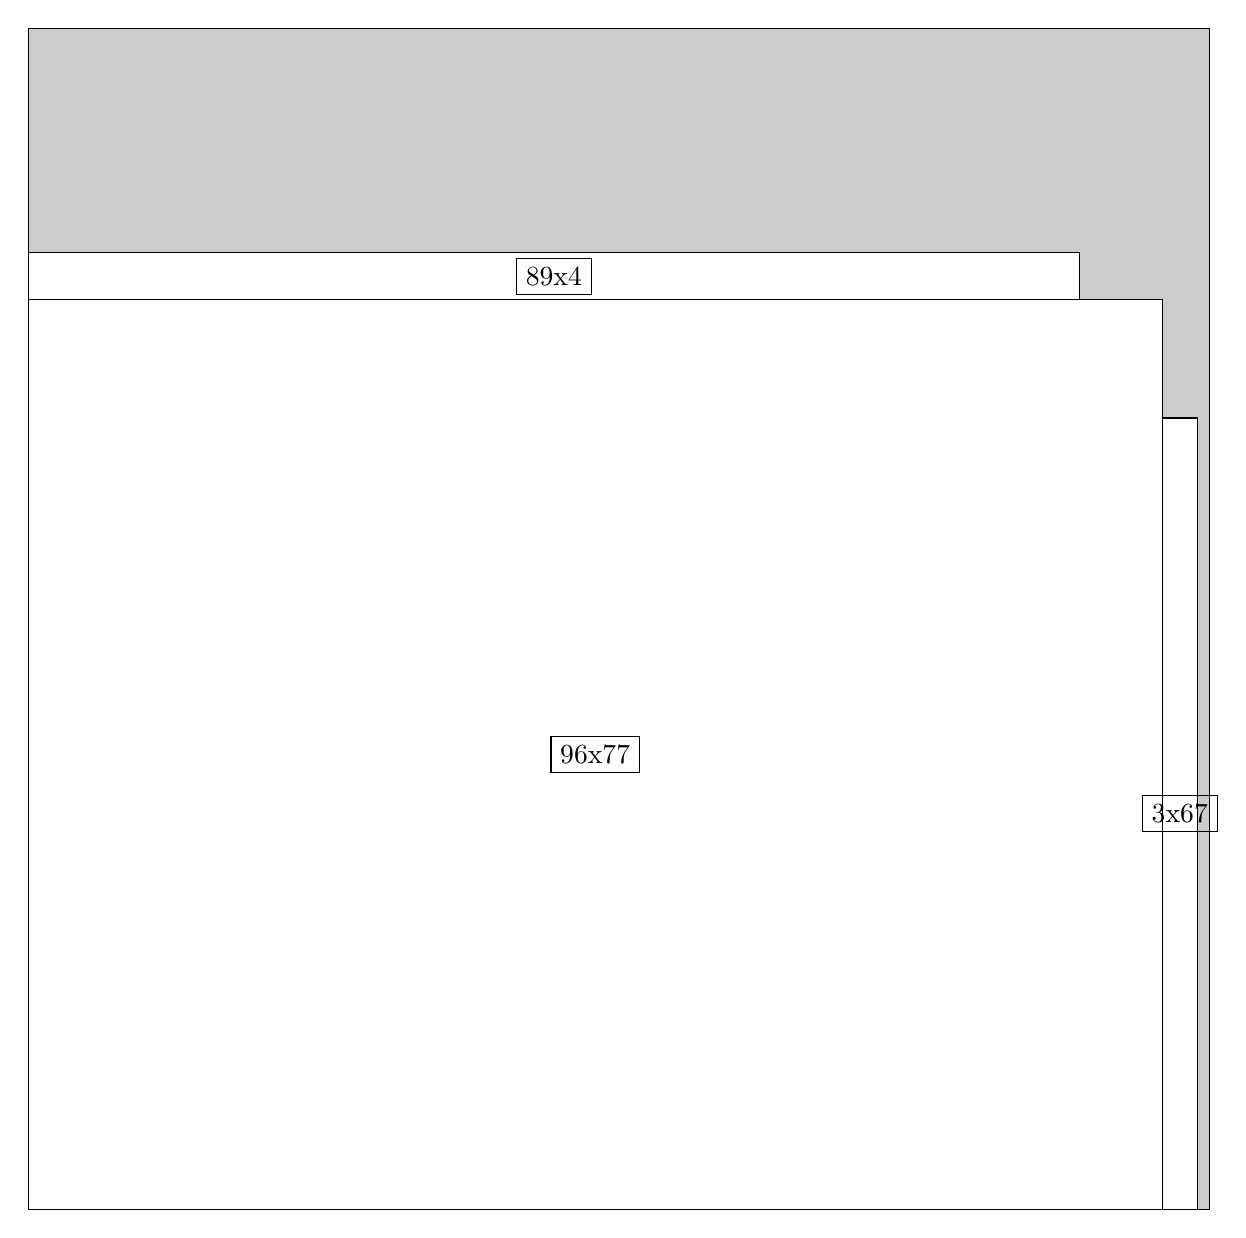
\begin{tikzpicture}[shorten >=1pt,scale=1.0,every node/.style={scale=1.0},->]
\tikzstyle{vertex}=[circle,fill=black!25,minimum size=14pt,inner sep=0pt]
\filldraw[fill=gray!40!white, draw=black] (0,0) rectangle (15.0,15.0);
\foreach \name/\x/\y/\w/\h in {96x77/0.0/0.0/14.399999999999999/11.549999999999999,89x4/0.0/11.549999999999999/13.35/0.6,3x67/14.399999999999999/0.0/0.44999999999999996/10.049999999999999}
\filldraw[fill=white!40!white, draw=black] (\x,\y) rectangle node[draw] (\name) {\name} ++(\w,\h);
\end{tikzpicture}


w =96 , h =77 , x =0 , y =0 , v =7392
\par
w =89 , h =4 , x =0 , y =77 , v =356
\par
w =3 , h =67 , x =96 , y =0 , v =201
\par
\newpage


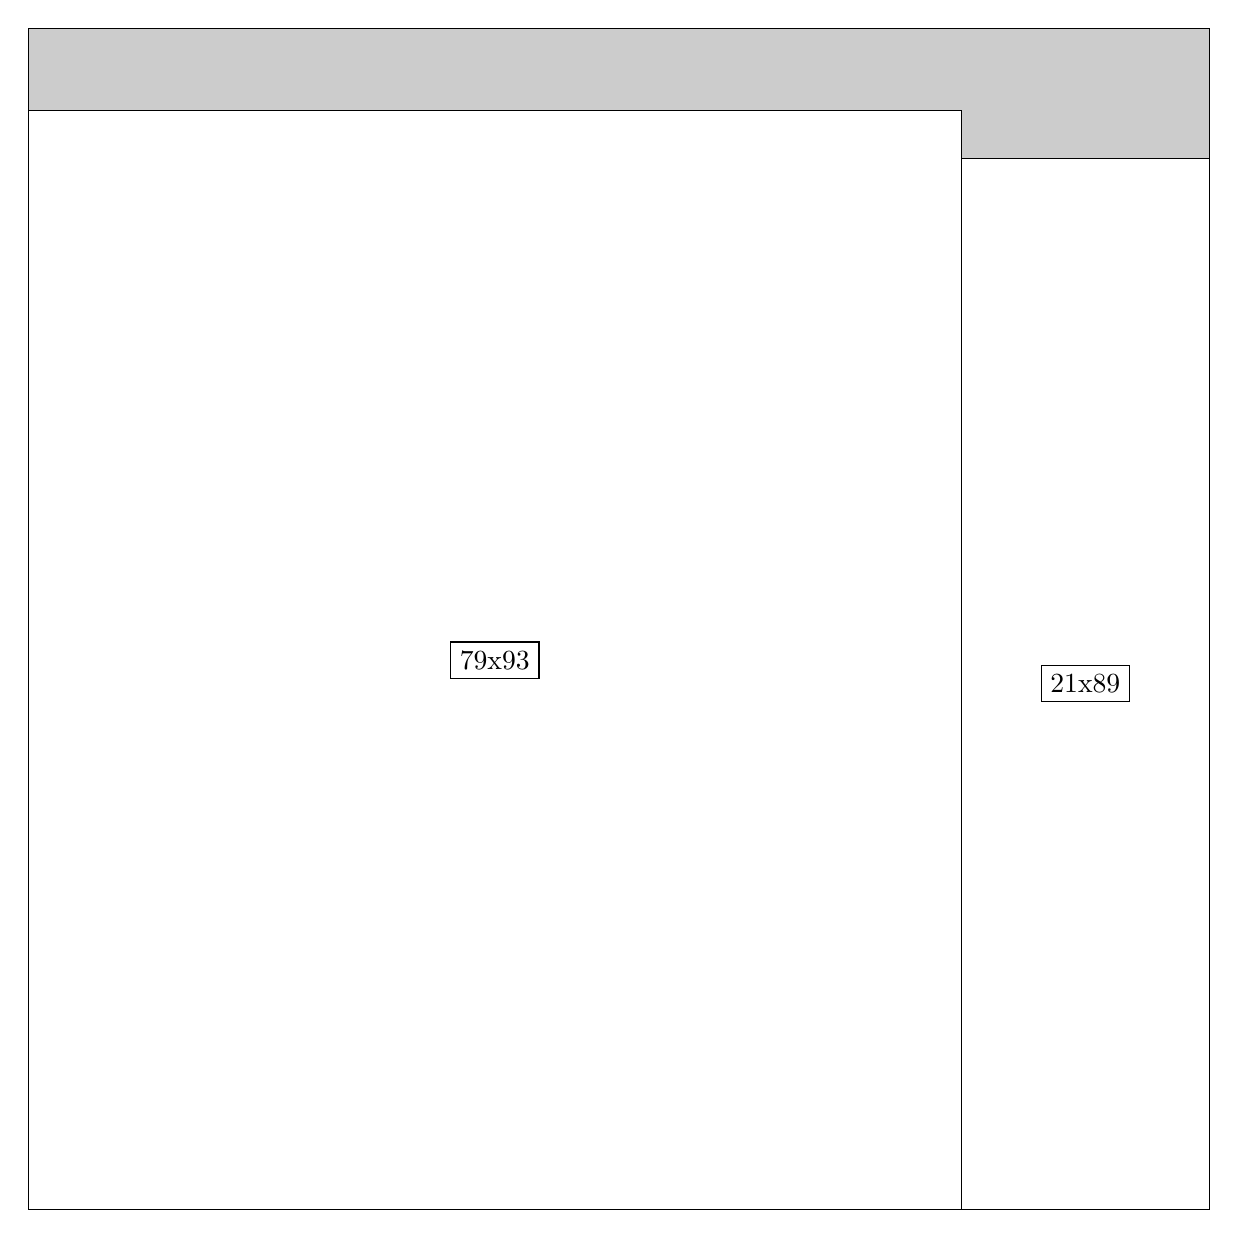
\begin{tikzpicture}[shorten >=1pt,scale=1.0,every node/.style={scale=1.0},->]
\tikzstyle{vertex}=[circle,fill=black!25,minimum size=14pt,inner sep=0pt]
\filldraw[fill=gray!40!white, draw=black] (0,0) rectangle (15.0,15.0);
\foreach \name/\x/\y/\w/\h in {79x93/0.0/0.0/11.85/13.95,21x89/11.85/0.0/3.15/13.35}
\filldraw[fill=white!40!white, draw=black] (\x,\y) rectangle node[draw] (\name) {\name} ++(\w,\h);
\end{tikzpicture}


w =79 , h =93 , x =0 , y =0 , v =7347
\par
w =21 , h =89 , x =79 , y =0 , v =1869
\par
\newpage


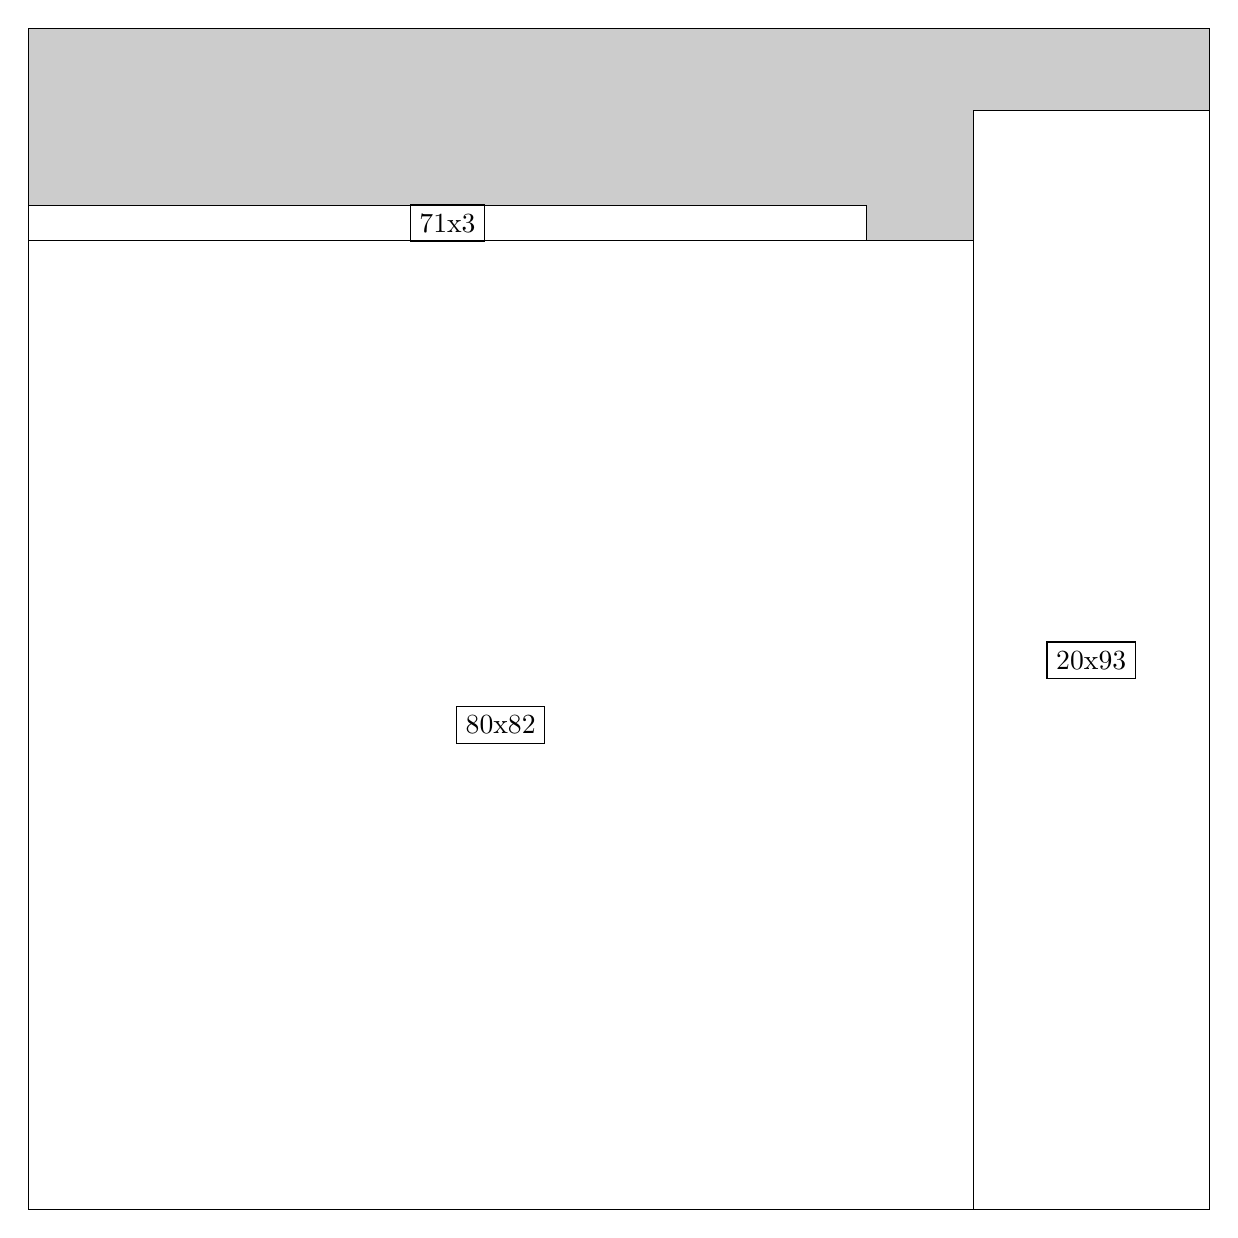
\begin{tikzpicture}[shorten >=1pt,scale=1.0,every node/.style={scale=1.0},->]
\tikzstyle{vertex}=[circle,fill=black!25,minimum size=14pt,inner sep=0pt]
\filldraw[fill=gray!40!white, draw=black] (0,0) rectangle (15.0,15.0);
\foreach \name/\x/\y/\w/\h in {80x82/0.0/0.0/12.0/12.299999999999999,20x93/12.0/0.0/3.0/13.95,71x3/0.0/12.299999999999999/10.65/0.44999999999999996}
\filldraw[fill=white!40!white, draw=black] (\x,\y) rectangle node[draw] (\name) {\name} ++(\w,\h);
\end{tikzpicture}


w =80 , h =82 , x =0 , y =0 , v =6560
\par
w =20 , h =93 , x =80 , y =0 , v =1860
\par
w =71 , h =3 , x =0 , y =82 , v =213
\par
\newpage


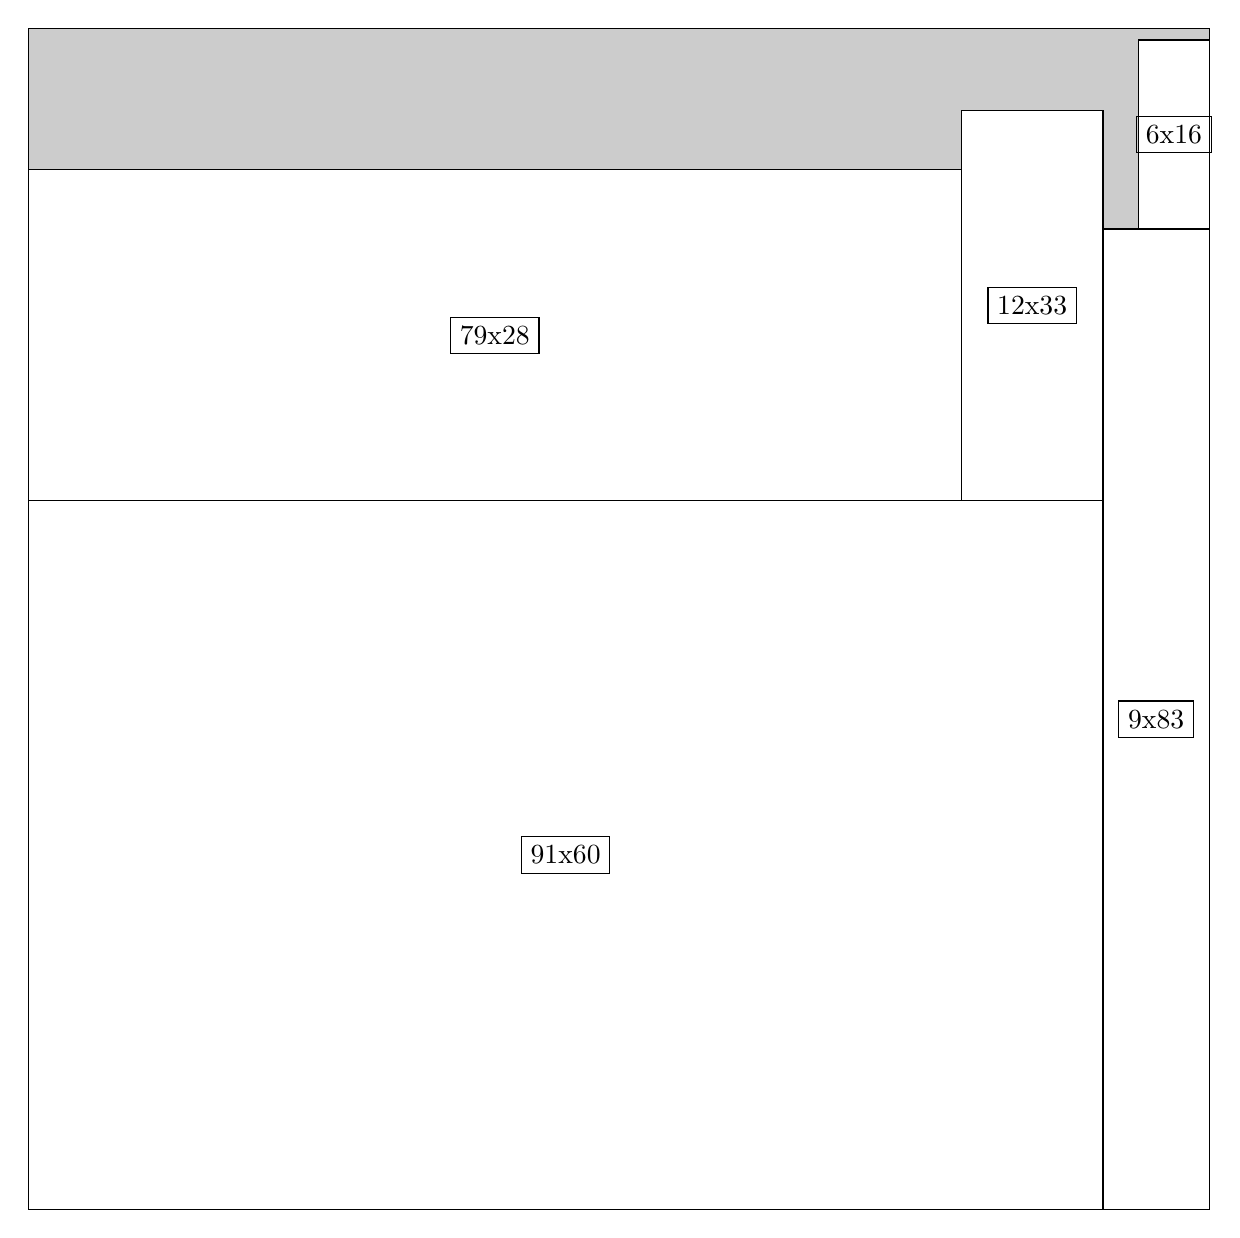
\begin{tikzpicture}[shorten >=1pt,scale=1.0,every node/.style={scale=1.0},->]
\tikzstyle{vertex}=[circle,fill=black!25,minimum size=14pt,inner sep=0pt]
\filldraw[fill=gray!40!white, draw=black] (0,0) rectangle (15.0,15.0);
\foreach \name/\x/\y/\w/\h in {91x60/0.0/0.0/13.65/9.0,79x28/0.0/9.0/11.85/4.2,9x83/13.65/0.0/1.3499999999999999/12.45,12x33/11.85/9.0/1.7999999999999998/4.95,6x16/14.1/12.45/0.8999999999999999/2.4}
\filldraw[fill=white!40!white, draw=black] (\x,\y) rectangle node[draw] (\name) {\name} ++(\w,\h);
\end{tikzpicture}


w =91 , h =60 , x =0 , y =0 , v =5460
\par
w =79 , h =28 , x =0 , y =60 , v =2212
\par
w =9 , h =83 , x =91 , y =0 , v =747
\par
w =12 , h =33 , x =79 , y =60 , v =396
\par
w =6 , h =16 , x =94 , y =83 , v =96
\par
\newpage


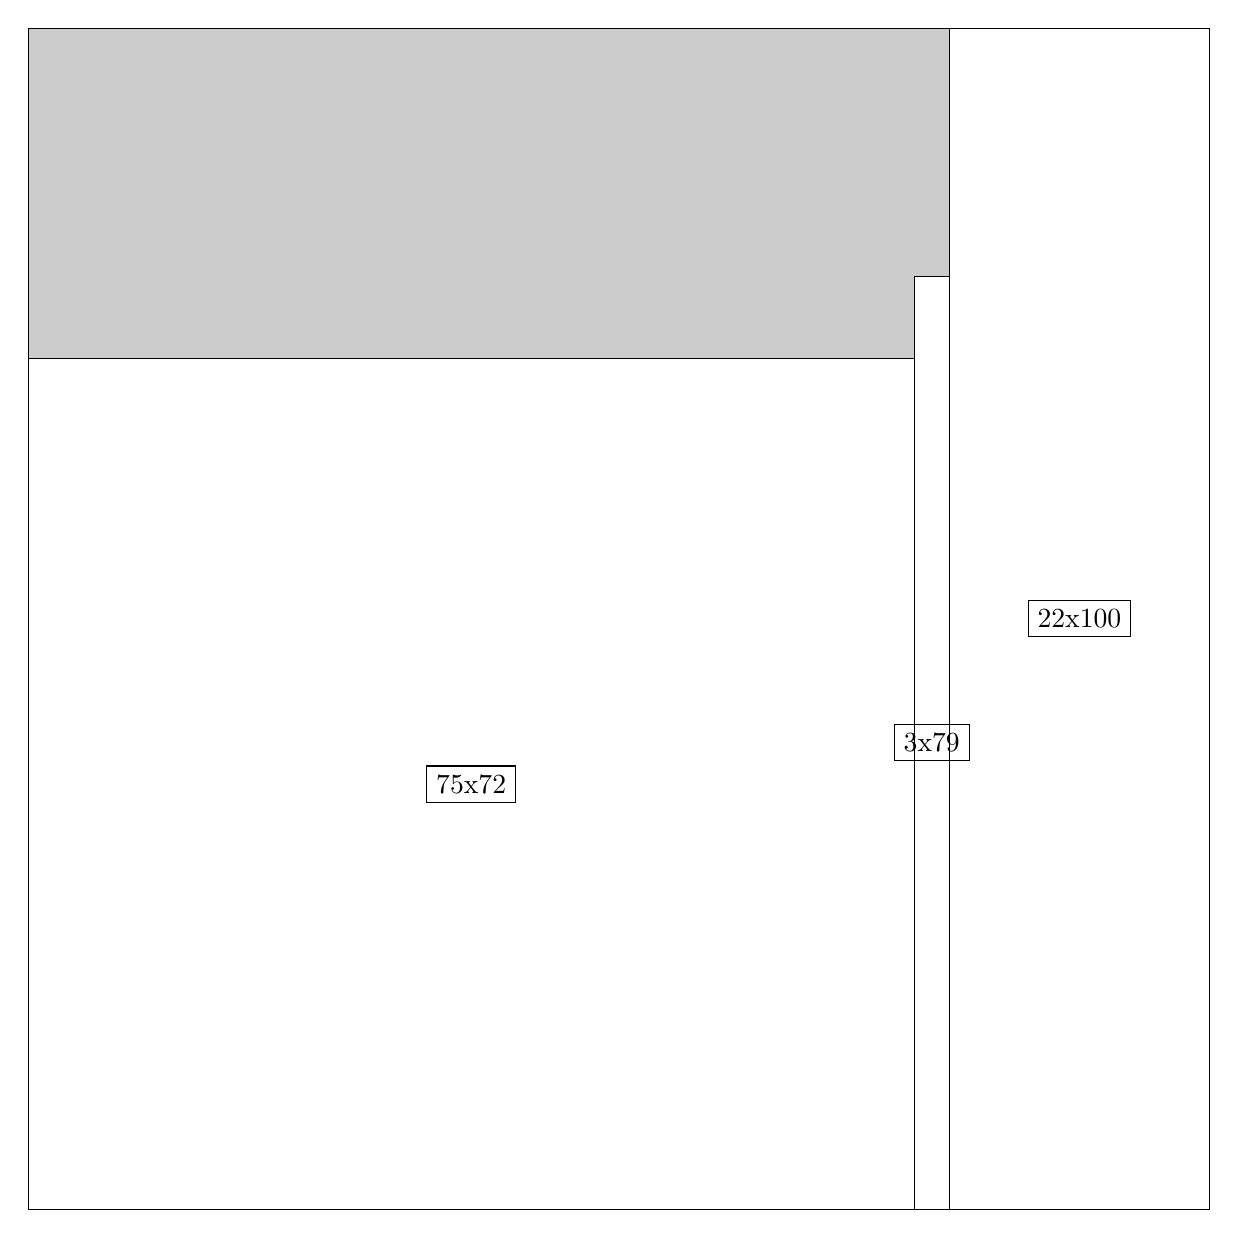
\begin{tikzpicture}[shorten >=1pt,scale=1.0,every node/.style={scale=1.0},->]
\tikzstyle{vertex}=[circle,fill=black!25,minimum size=14pt,inner sep=0pt]
\filldraw[fill=gray!40!white, draw=black] (0,0) rectangle (15.0,15.0);
\foreach \name/\x/\y/\w/\h in {75x72/0.0/0.0/11.25/10.799999999999999,22x100/11.7/0.0/3.3/15.0,3x79/11.25/0.0/0.44999999999999996/11.85}
\filldraw[fill=white!40!white, draw=black] (\x,\y) rectangle node[draw] (\name) {\name} ++(\w,\h);
\end{tikzpicture}


w =75 , h =72 , x =0 , y =0 , v =5400
\par
w =22 , h =100 , x =78 , y =0 , v =2200
\par
w =3 , h =79 , x =75 , y =0 , v =237
\par
\newpage


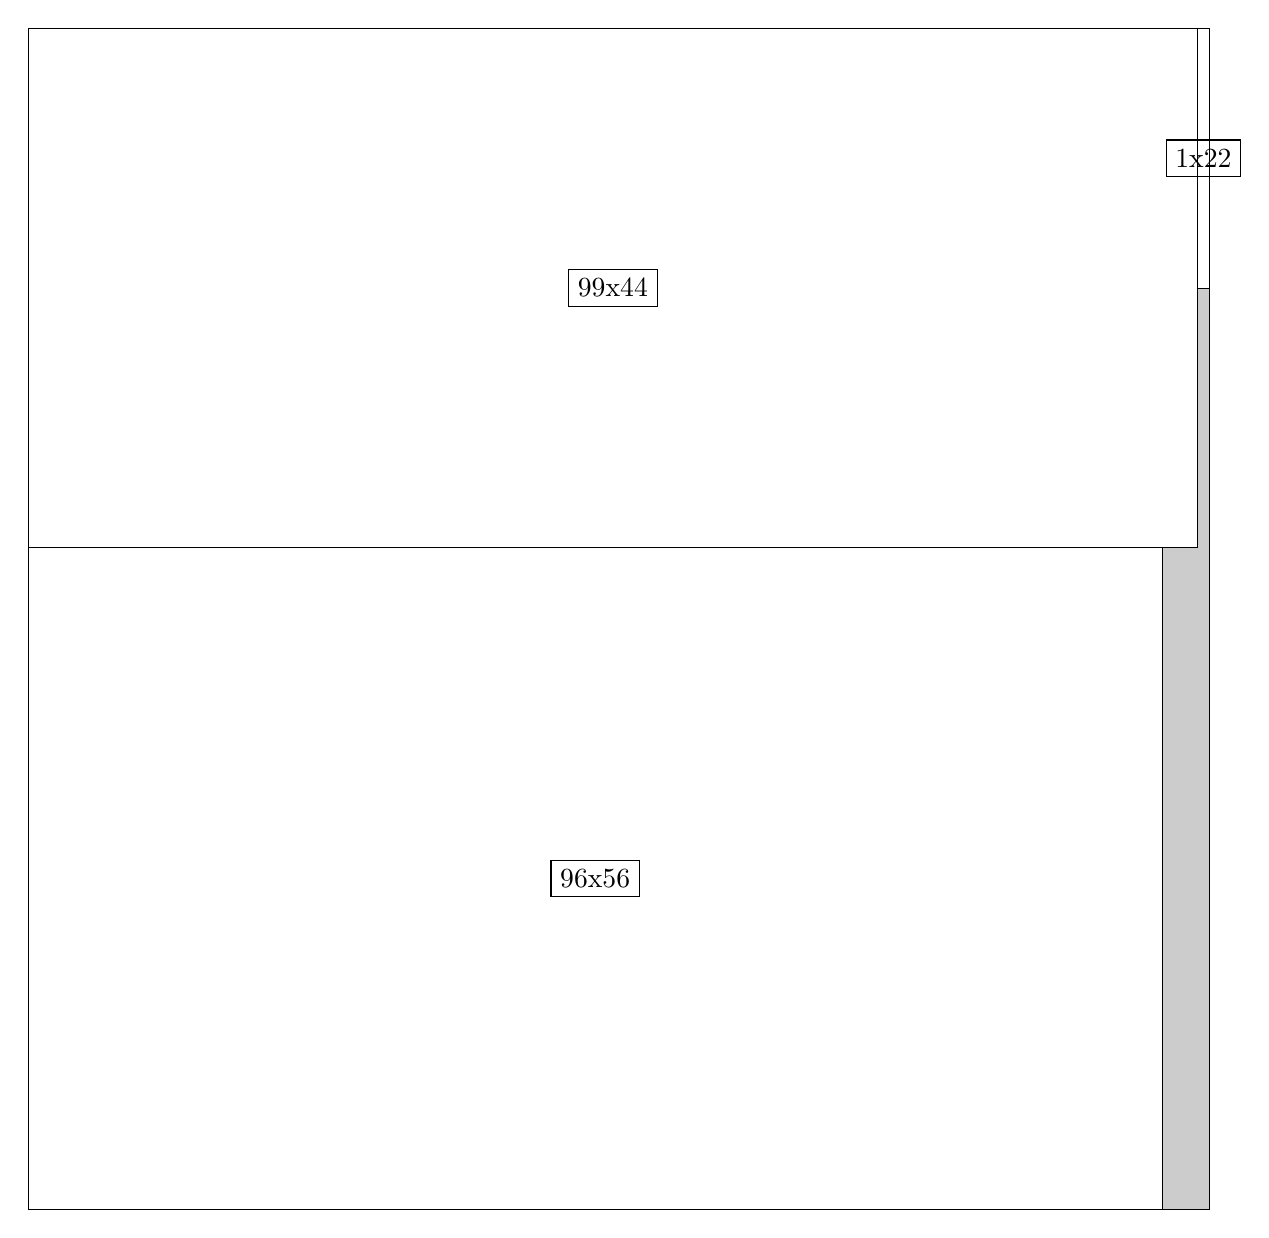
\begin{tikzpicture}[shorten >=1pt,scale=1.0,every node/.style={scale=1.0},->]
\tikzstyle{vertex}=[circle,fill=black!25,minimum size=14pt,inner sep=0pt]
\filldraw[fill=gray!40!white, draw=black] (0,0) rectangle (15.0,15.0);
\foreach \name/\x/\y/\w/\h in {96x56/0.0/0.0/14.399999999999999/8.4,99x44/0.0/8.4/14.85/6.6,1x22/14.85/11.7/0.15/3.3}
\filldraw[fill=white!40!white, draw=black] (\x,\y) rectangle node[draw] (\name) {\name} ++(\w,\h);
\end{tikzpicture}


w =96 , h =56 , x =0 , y =0 , v =5376
\par
w =99 , h =44 , x =0 , y =56 , v =4356
\par
w =1 , h =22 , x =99 , y =78 , v =22
\par
\newpage


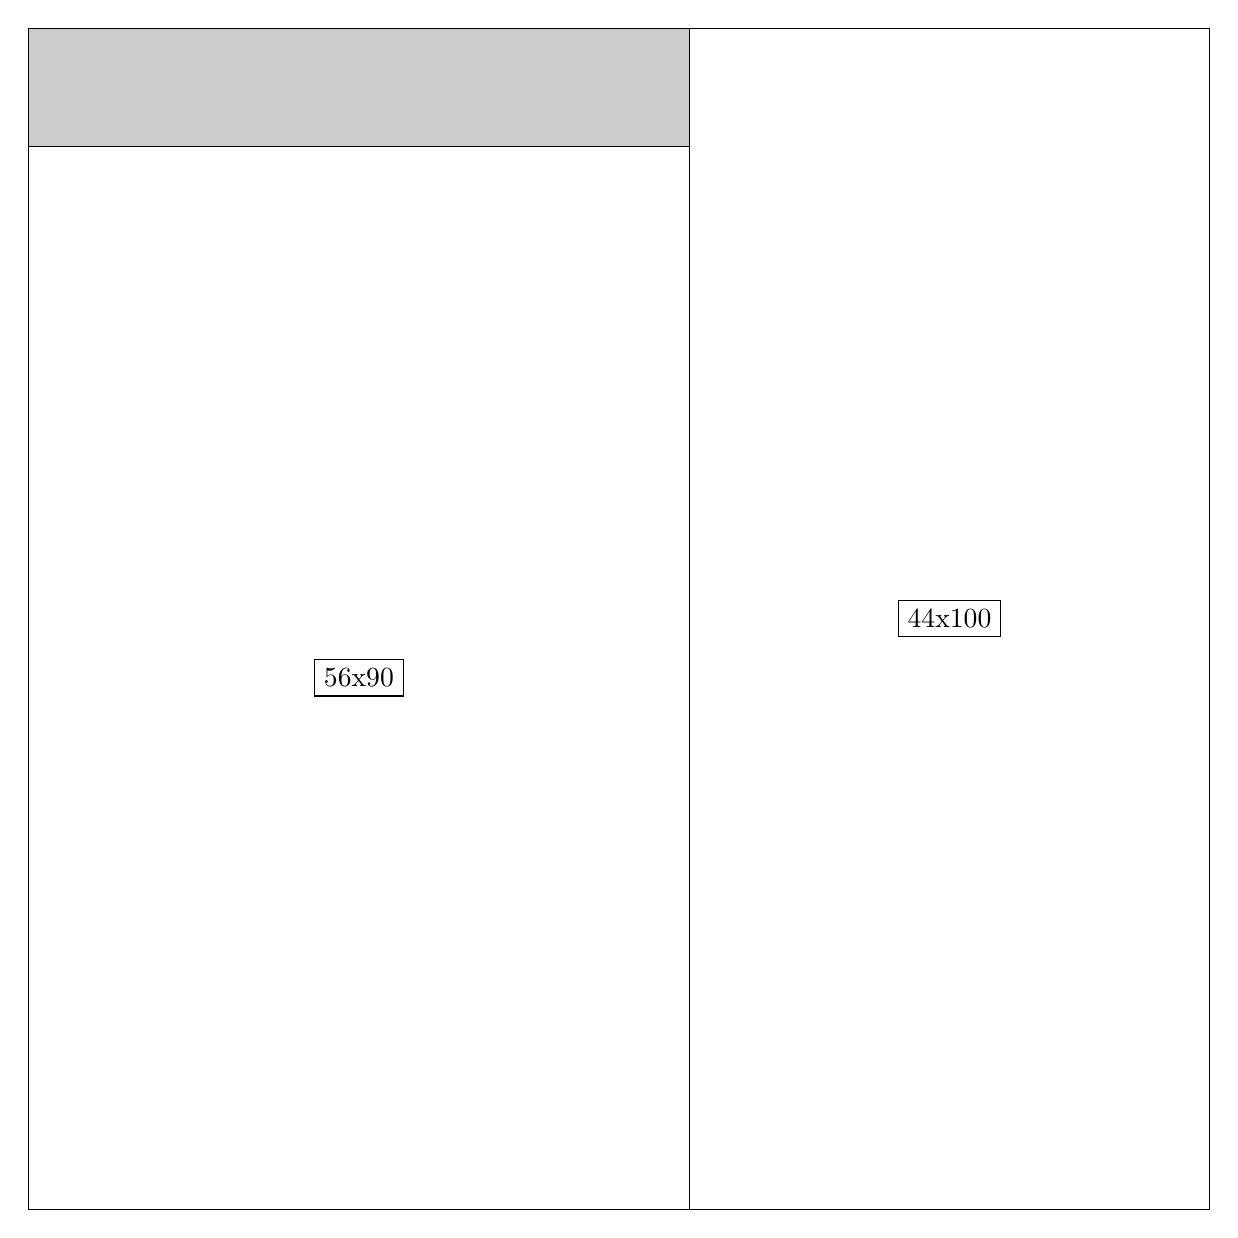
\begin{tikzpicture}[shorten >=1pt,scale=1.0,every node/.style={scale=1.0},->]
\tikzstyle{vertex}=[circle,fill=black!25,minimum size=14pt,inner sep=0pt]
\filldraw[fill=gray!40!white, draw=black] (0,0) rectangle (15.0,15.0);
\foreach \name/\x/\y/\w/\h in {56x90/0.0/0.0/8.4/13.5,44x100/8.4/0.0/6.6/15.0}
\filldraw[fill=white!40!white, draw=black] (\x,\y) rectangle node[draw] (\name) {\name} ++(\w,\h);
\end{tikzpicture}


w =56 , h =90 , x =0 , y =0 , v =5040
\par
w =44 , h =100 , x =56 , y =0 , v =4400
\par
\newpage


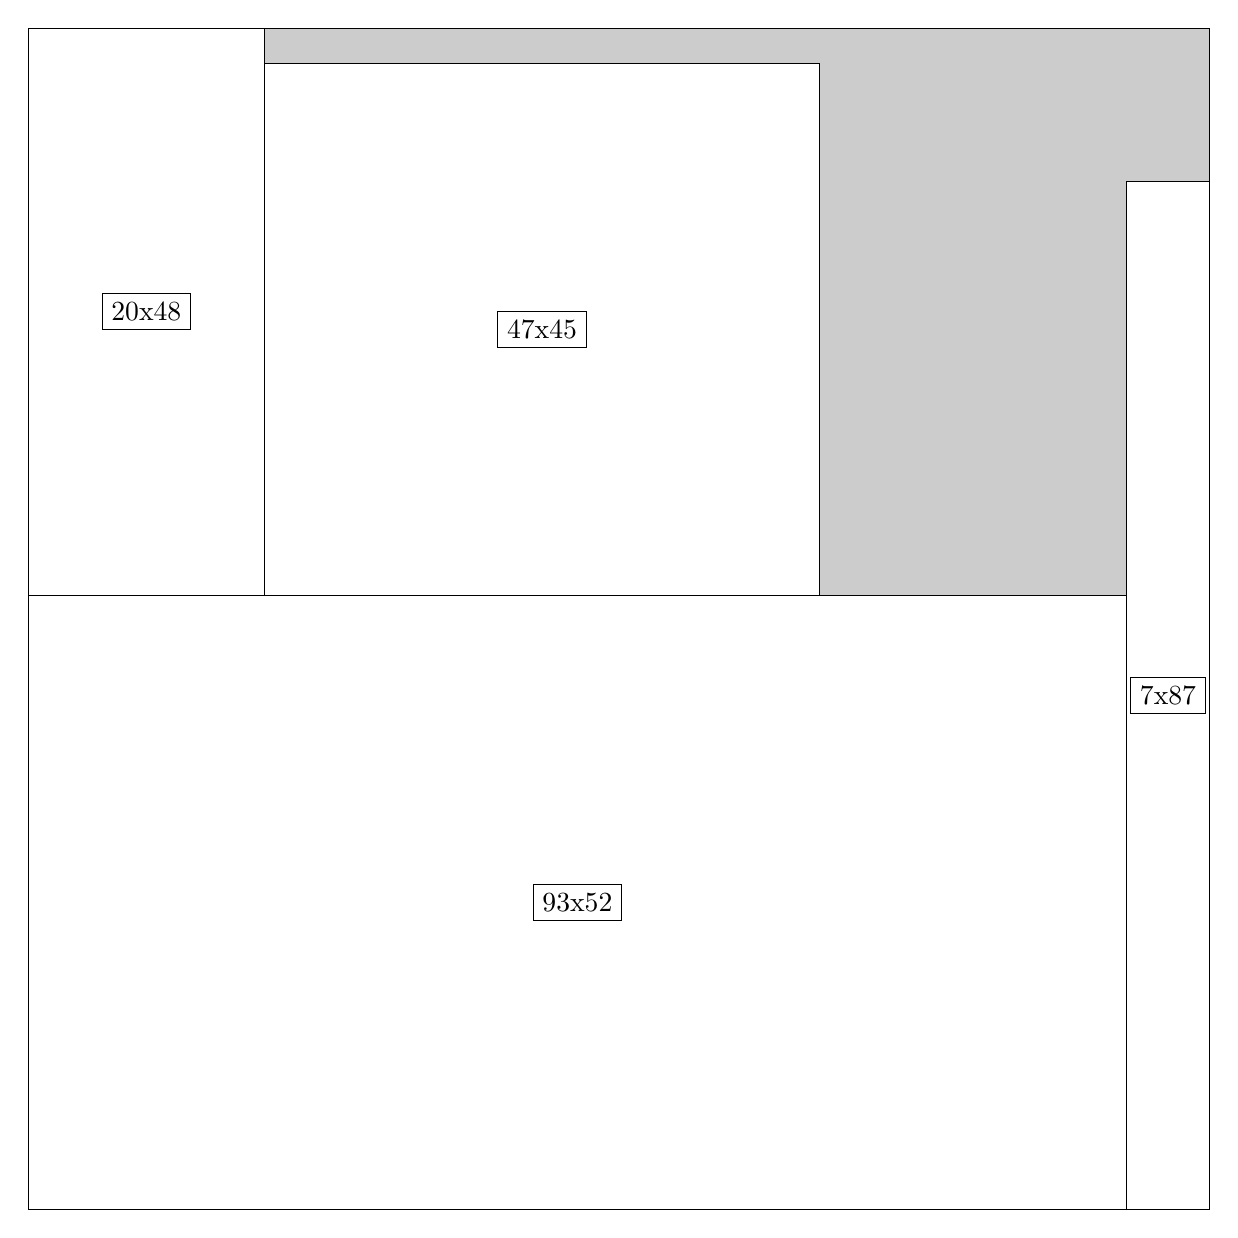
\begin{tikzpicture}[shorten >=1pt,scale=1.0,every node/.style={scale=1.0},->]
\tikzstyle{vertex}=[circle,fill=black!25,minimum size=14pt,inner sep=0pt]
\filldraw[fill=gray!40!white, draw=black] (0,0) rectangle (15.0,15.0);
\foreach \name/\x/\y/\w/\h in {93x52/0.0/0.0/13.95/7.8,47x45/3.0/7.8/7.05/6.75,20x48/0.0/7.8/3.0/7.199999999999999,7x87/13.95/0.0/1.05/13.049999999999999}
\filldraw[fill=white!40!white, draw=black] (\x,\y) rectangle node[draw] (\name) {\name} ++(\w,\h);
\end{tikzpicture}


w =93 , h =52 , x =0 , y =0 , v =4836
\par
w =47 , h =45 , x =20 , y =52 , v =2115
\par
w =20 , h =48 , x =0 , y =52 , v =960
\par
w =7 , h =87 , x =93 , y =0 , v =609
\par
\newpage


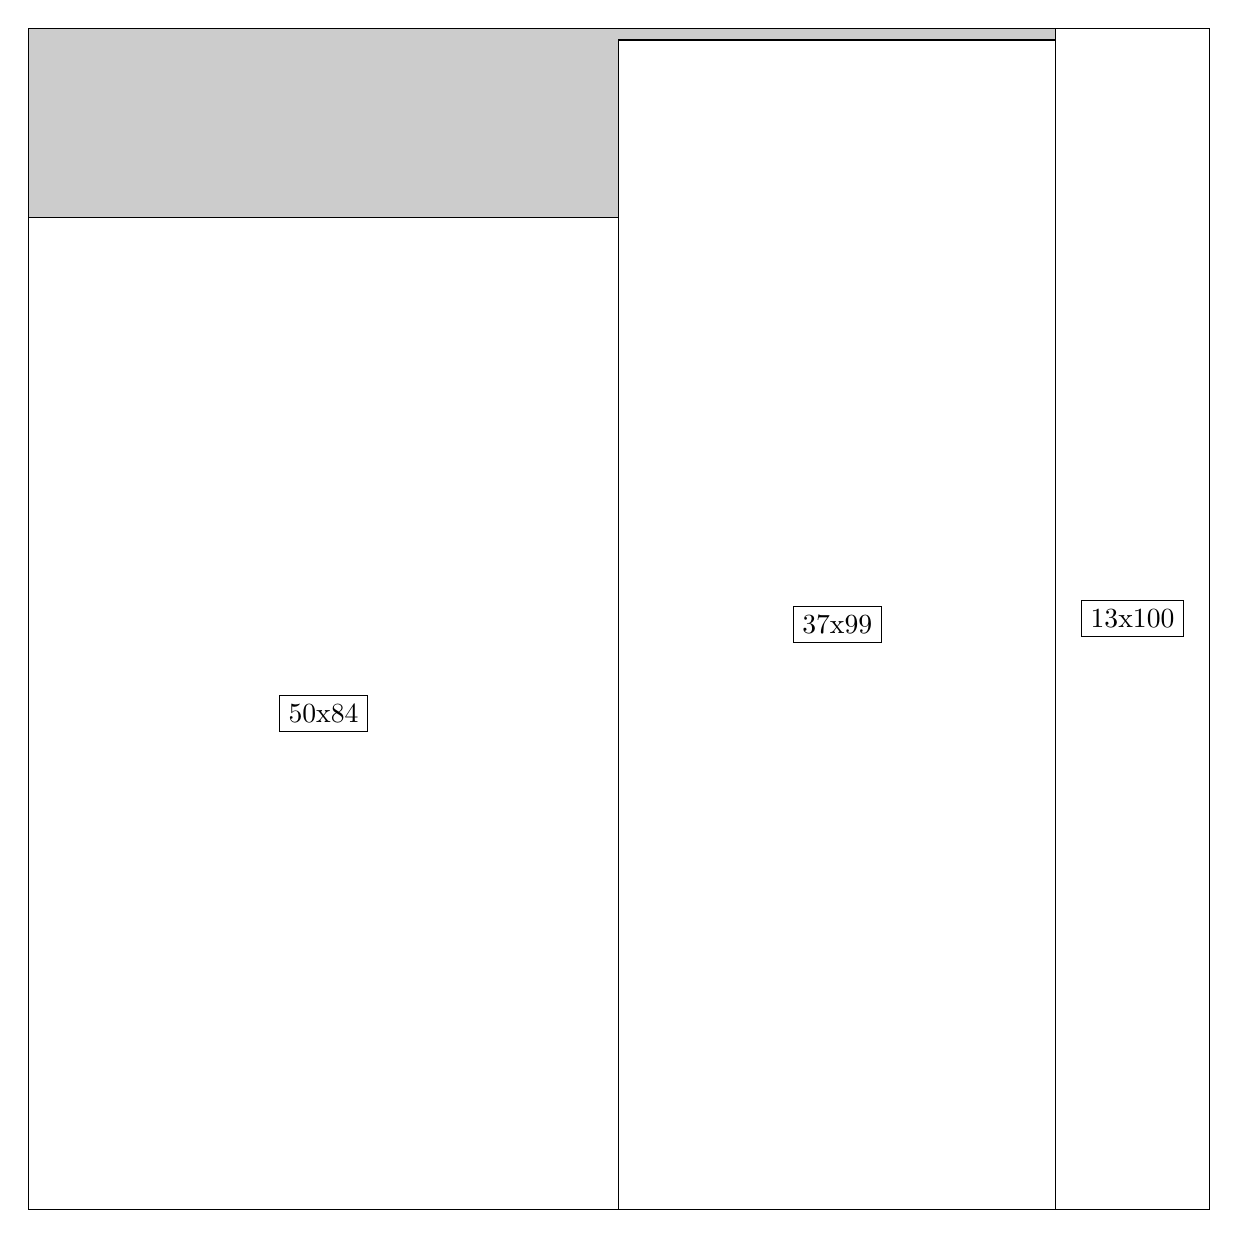
\begin{tikzpicture}[shorten >=1pt,scale=1.0,every node/.style={scale=1.0},->]
\tikzstyle{vertex}=[circle,fill=black!25,minimum size=14pt,inner sep=0pt]
\filldraw[fill=gray!40!white, draw=black] (0,0) rectangle (15.0,15.0);
\foreach \name/\x/\y/\w/\h in {50x84/0.0/0.0/7.5/12.6,37x99/7.5/0.0/5.55/14.85,13x100/13.049999999999999/0.0/1.95/15.0}
\filldraw[fill=white!40!white, draw=black] (\x,\y) rectangle node[draw] (\name) {\name} ++(\w,\h);
\end{tikzpicture}


w =50 , h =84 , x =0 , y =0 , v =4200
\par
w =37 , h =99 , x =50 , y =0 , v =3663
\par
w =13 , h =100 , x =87 , y =0 , v =1300
\par
\newpage


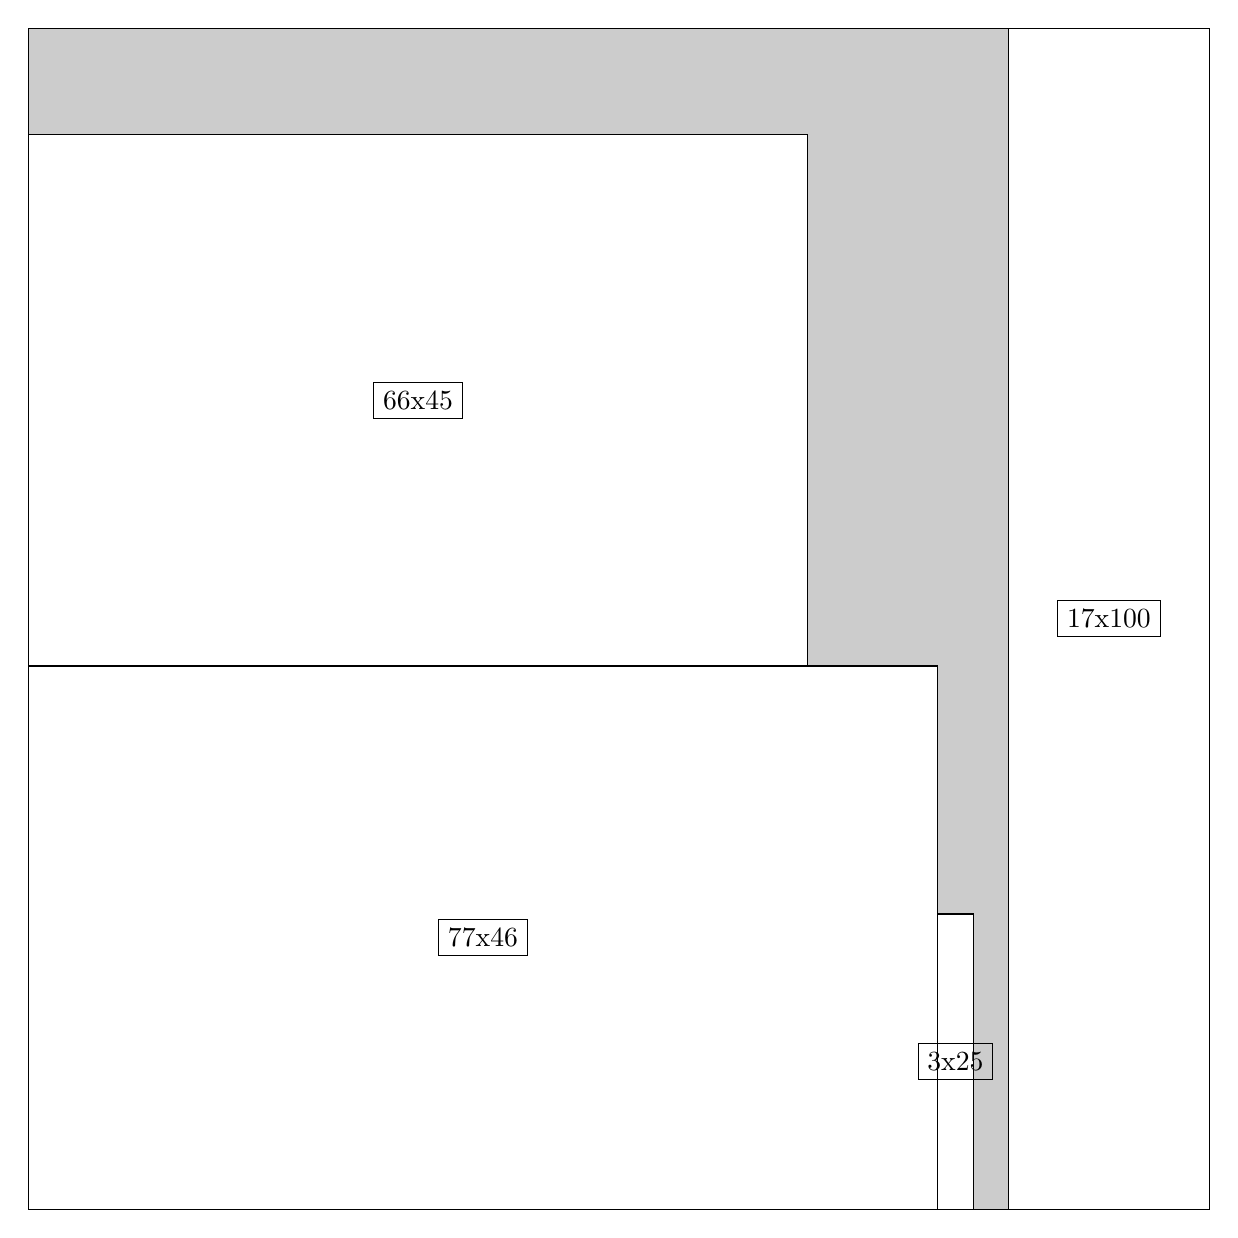
\begin{tikzpicture}[shorten >=1pt,scale=1.0,every node/.style={scale=1.0},->]
\tikzstyle{vertex}=[circle,fill=black!25,minimum size=14pt,inner sep=0pt]
\filldraw[fill=gray!40!white, draw=black] (0,0) rectangle (15.0,15.0);
\foreach \name/\x/\y/\w/\h in {77x46/0.0/0.0/11.549999999999999/6.8999999999999995,3x25/11.549999999999999/0.0/0.44999999999999996/3.75,17x100/12.45/0.0/2.55/15.0,66x45/0.0/6.8999999999999995/9.9/6.75}
\filldraw[fill=white!40!white, draw=black] (\x,\y) rectangle node[draw] (\name) {\name} ++(\w,\h);
\end{tikzpicture}


w =77 , h =46 , x =0 , y =0 , v =3542
\par
w =3 , h =25 , x =77 , y =0 , v =75
\par
w =17 , h =100 , x =83 , y =0 , v =1700
\par
w =66 , h =45 , x =0 , y =46 , v =2970
\par
\newpage


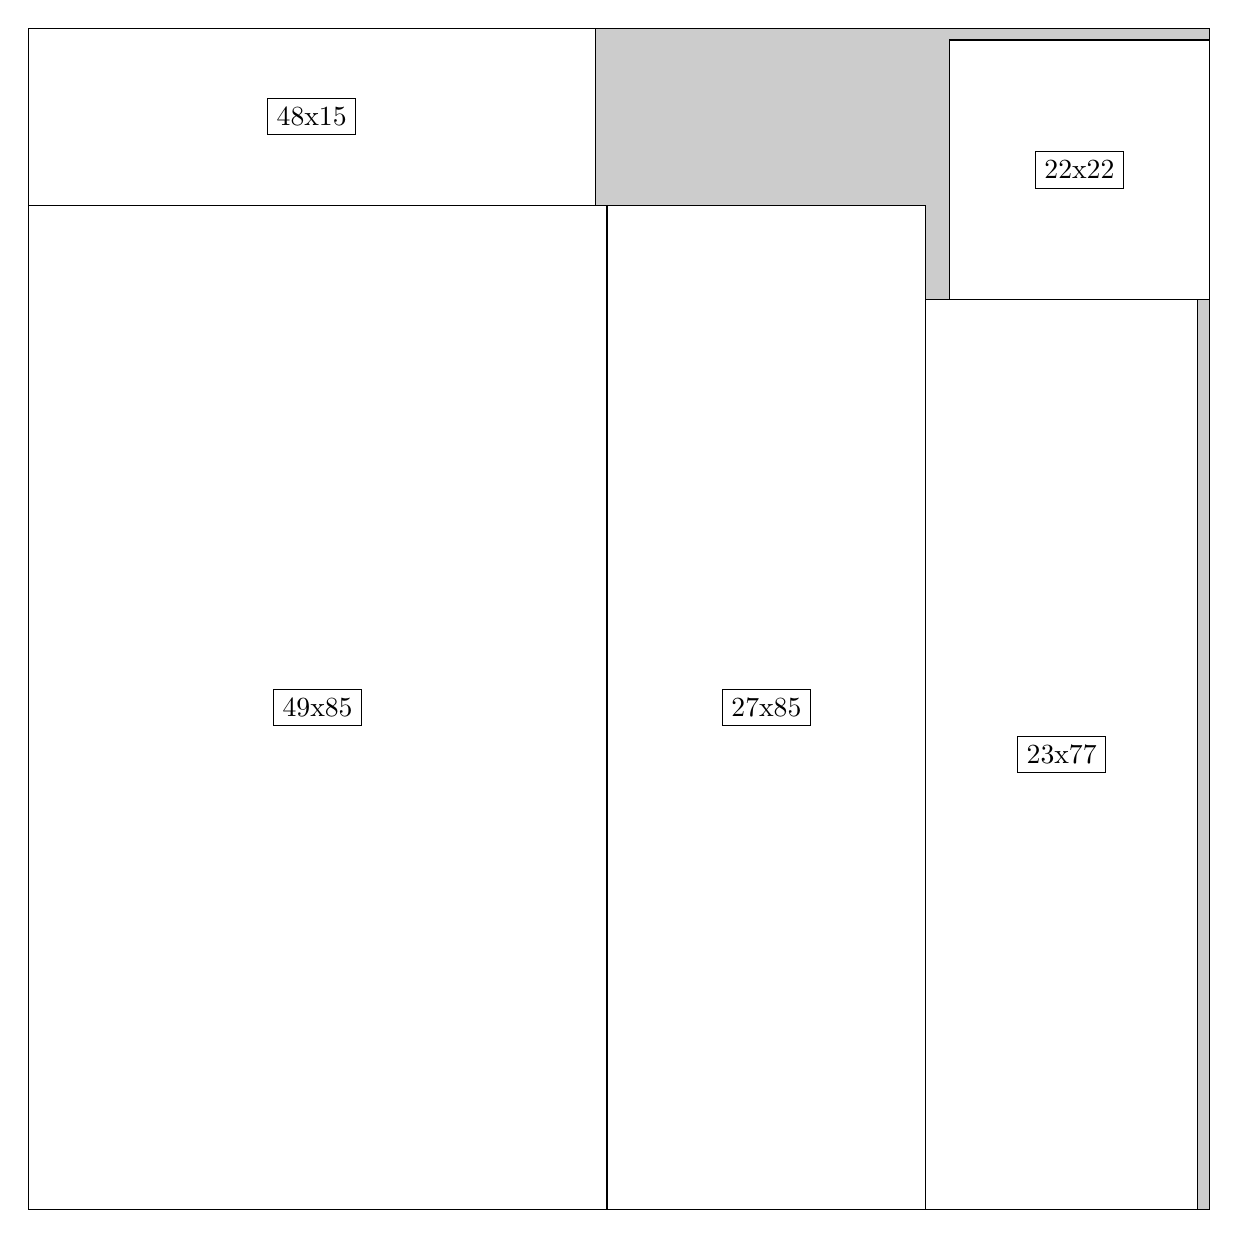
\begin{tikzpicture}[shorten >=1pt,scale=1.0,every node/.style={scale=1.0},->]
\tikzstyle{vertex}=[circle,fill=black!25,minimum size=14pt,inner sep=0pt]
\filldraw[fill=gray!40!white, draw=black] (0,0) rectangle (15.0,15.0);
\foreach \name/\x/\y/\w/\h in {49x85/0.0/0.0/7.35/12.75,27x85/7.35/0.0/4.05/12.75,23x77/11.4/0.0/3.4499999999999997/11.549999999999999,48x15/0.0/12.75/7.199999999999999/2.25,22x22/11.7/11.549999999999999/3.3/3.3}
\filldraw[fill=white!40!white, draw=black] (\x,\y) rectangle node[draw] (\name) {\name} ++(\w,\h);
\end{tikzpicture}


w =49 , h =85 , x =0 , y =0 , v =4165
\par
w =27 , h =85 , x =49 , y =0 , v =2295
\par
w =23 , h =77 , x =76 , y =0 , v =1771
\par
w =48 , h =15 , x =0 , y =85 , v =720
\par
w =22 , h =22 , x =78 , y =77 , v =484
\par
\newpage


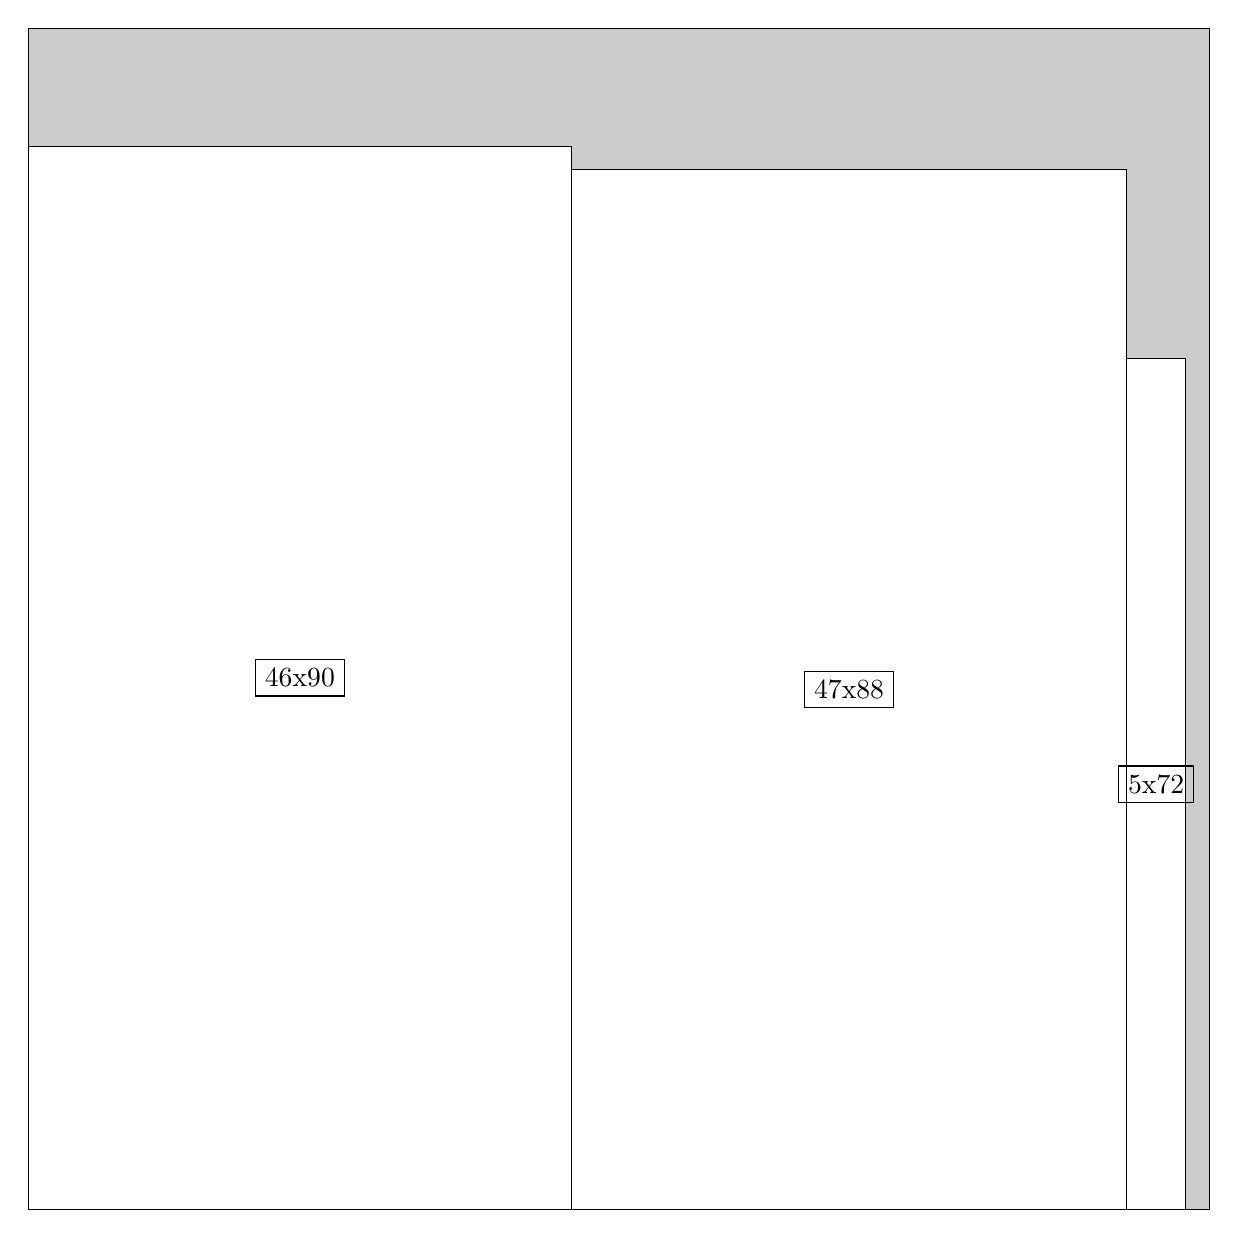
\begin{tikzpicture}[shorten >=1pt,scale=1.0,every node/.style={scale=1.0},->]
\tikzstyle{vertex}=[circle,fill=black!25,minimum size=14pt,inner sep=0pt]
\filldraw[fill=gray!40!white, draw=black] (0,0) rectangle (15.0,15.0);
\foreach \name/\x/\y/\w/\h in {46x90/0.0/0.0/6.8999999999999995/13.5,47x88/6.8999999999999995/0.0/7.05/13.2,5x72/13.95/0.0/0.75/10.799999999999999}
\filldraw[fill=white!40!white, draw=black] (\x,\y) rectangle node[draw] (\name) {\name} ++(\w,\h);
\end{tikzpicture}


w =46 , h =90 , x =0 , y =0 , v =4140
\par
w =47 , h =88 , x =46 , y =0 , v =4136
\par
w =5 , h =72 , x =93 , y =0 , v =360
\par
\newpage


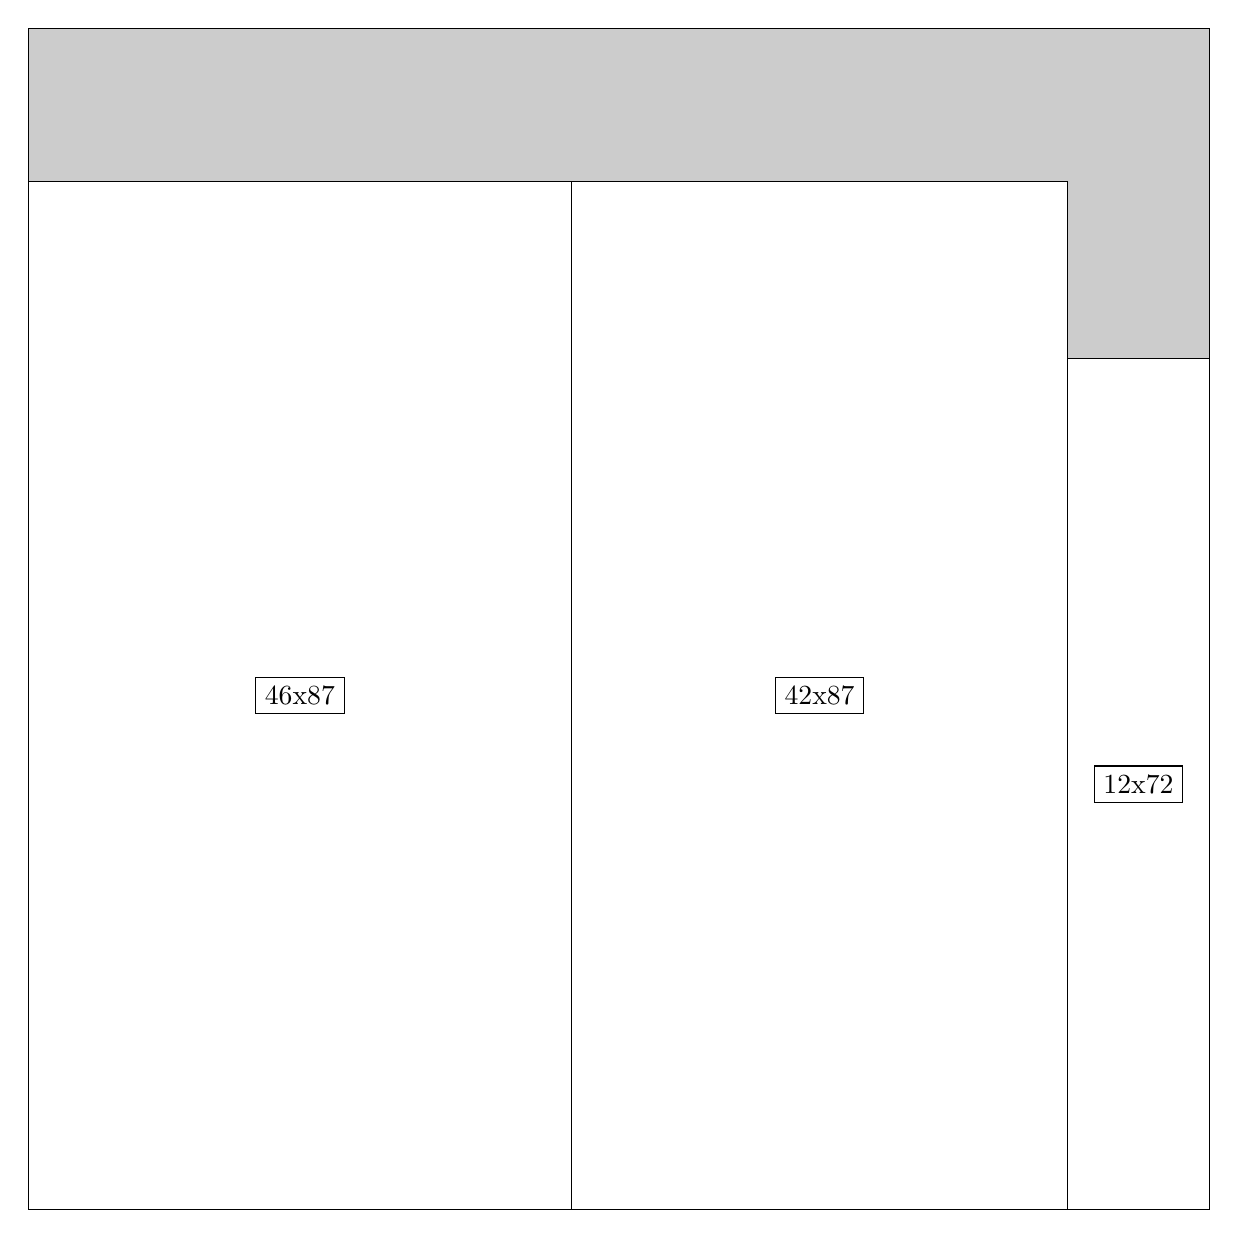
\begin{tikzpicture}[shorten >=1pt,scale=1.0,every node/.style={scale=1.0},->]
\tikzstyle{vertex}=[circle,fill=black!25,minimum size=14pt,inner sep=0pt]
\filldraw[fill=gray!40!white, draw=black] (0,0) rectangle (15.0,15.0);
\foreach \name/\x/\y/\w/\h in {46x87/0.0/0.0/6.8999999999999995/13.049999999999999,42x87/6.8999999999999995/0.0/6.3/13.049999999999999,12x72/13.2/0.0/1.7999999999999998/10.799999999999999}
\filldraw[fill=white!40!white, draw=black] (\x,\y) rectangle node[draw] (\name) {\name} ++(\w,\h);
\end{tikzpicture}


w =46 , h =87 , x =0 , y =0 , v =4002
\par
w =42 , h =87 , x =46 , y =0 , v =3654
\par
w =12 , h =72 , x =88 , y =0 , v =864
\par
\newpage


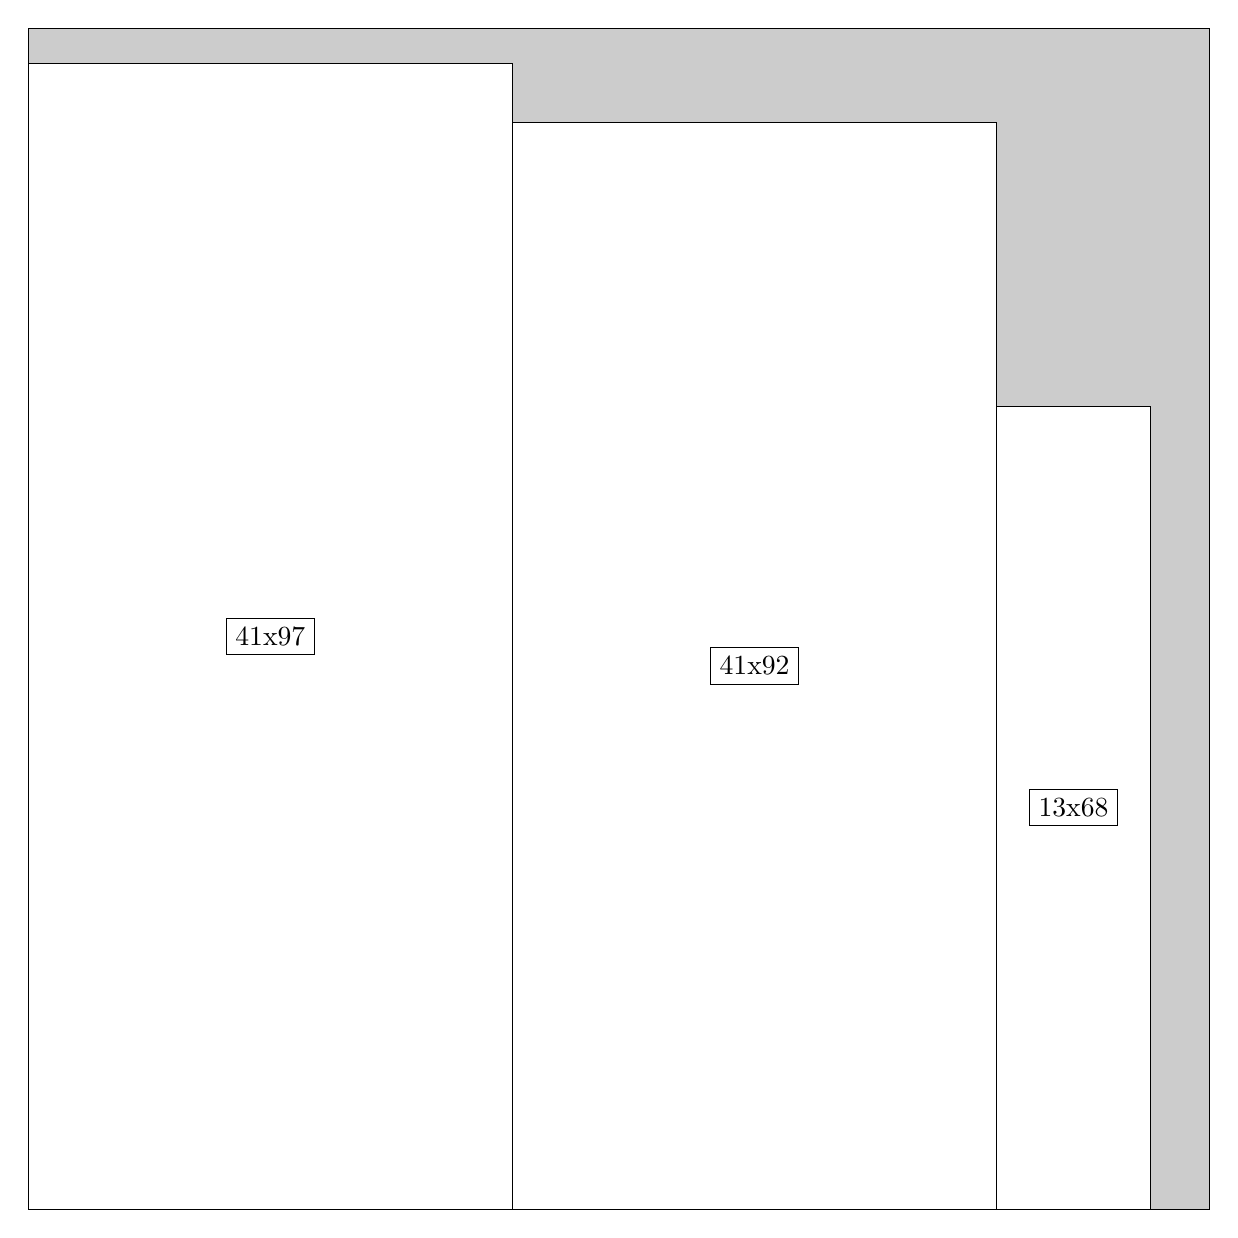
\begin{tikzpicture}[shorten >=1pt,scale=1.0,every node/.style={scale=1.0},->]
\tikzstyle{vertex}=[circle,fill=black!25,minimum size=14pt,inner sep=0pt]
\filldraw[fill=gray!40!white, draw=black] (0,0) rectangle (15.0,15.0);
\foreach \name/\x/\y/\w/\h in {41x97/0.0/0.0/6.1499999999999995/14.549999999999999,41x92/6.1499999999999995/0.0/6.1499999999999995/13.799999999999999,13x68/12.299999999999999/0.0/1.95/10.2}
\filldraw[fill=white!40!white, draw=black] (\x,\y) rectangle node[draw] (\name) {\name} ++(\w,\h);
\end{tikzpicture}


w =41 , h =97 , x =0 , y =0 , v =3977
\par
w =41 , h =92 , x =41 , y =0 , v =3772
\par
w =13 , h =68 , x =82 , y =0 , v =884
\par
\newpage


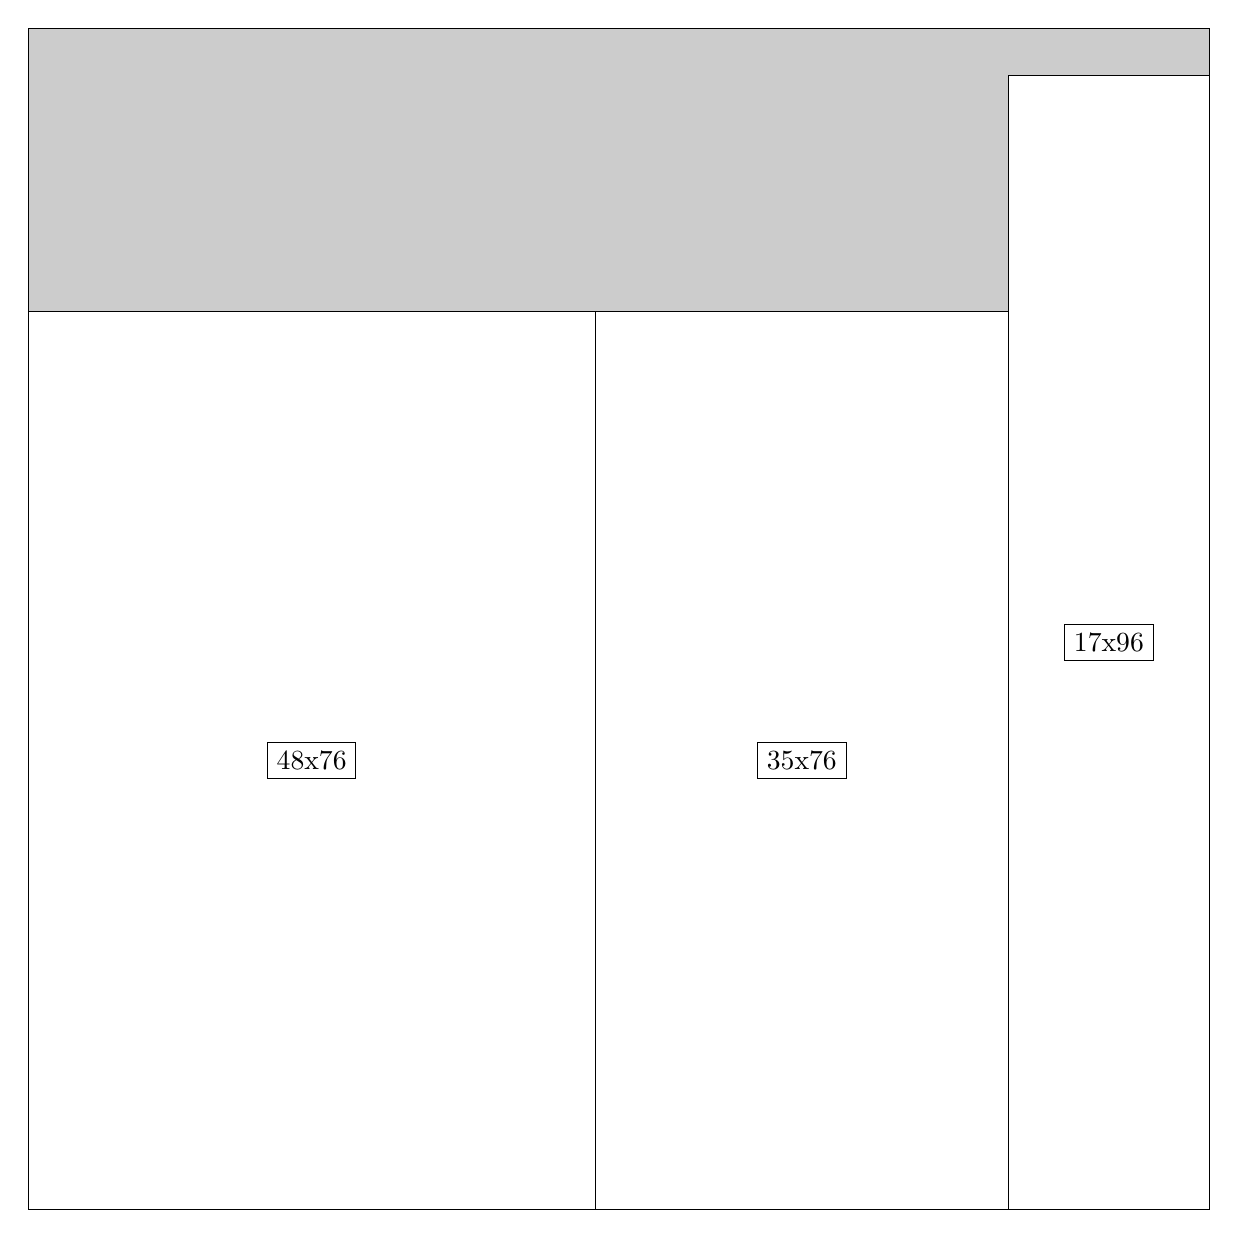
\begin{tikzpicture}[shorten >=1pt,scale=1.0,every node/.style={scale=1.0},->]
\tikzstyle{vertex}=[circle,fill=black!25,minimum size=14pt,inner sep=0pt]
\filldraw[fill=gray!40!white, draw=black] (0,0) rectangle (15.0,15.0);
\foreach \name/\x/\y/\w/\h in {48x76/0.0/0.0/7.199999999999999/11.4,35x76/7.199999999999999/0.0/5.25/11.4,17x96/12.45/0.0/2.55/14.399999999999999}
\filldraw[fill=white!40!white, draw=black] (\x,\y) rectangle node[draw] (\name) {\name} ++(\w,\h);
\end{tikzpicture}


w =48 , h =76 , x =0 , y =0 , v =3648
\par
w =35 , h =76 , x =48 , y =0 , v =2660
\par
w =17 , h =96 , x =83 , y =0 , v =1632
\par
\newpage


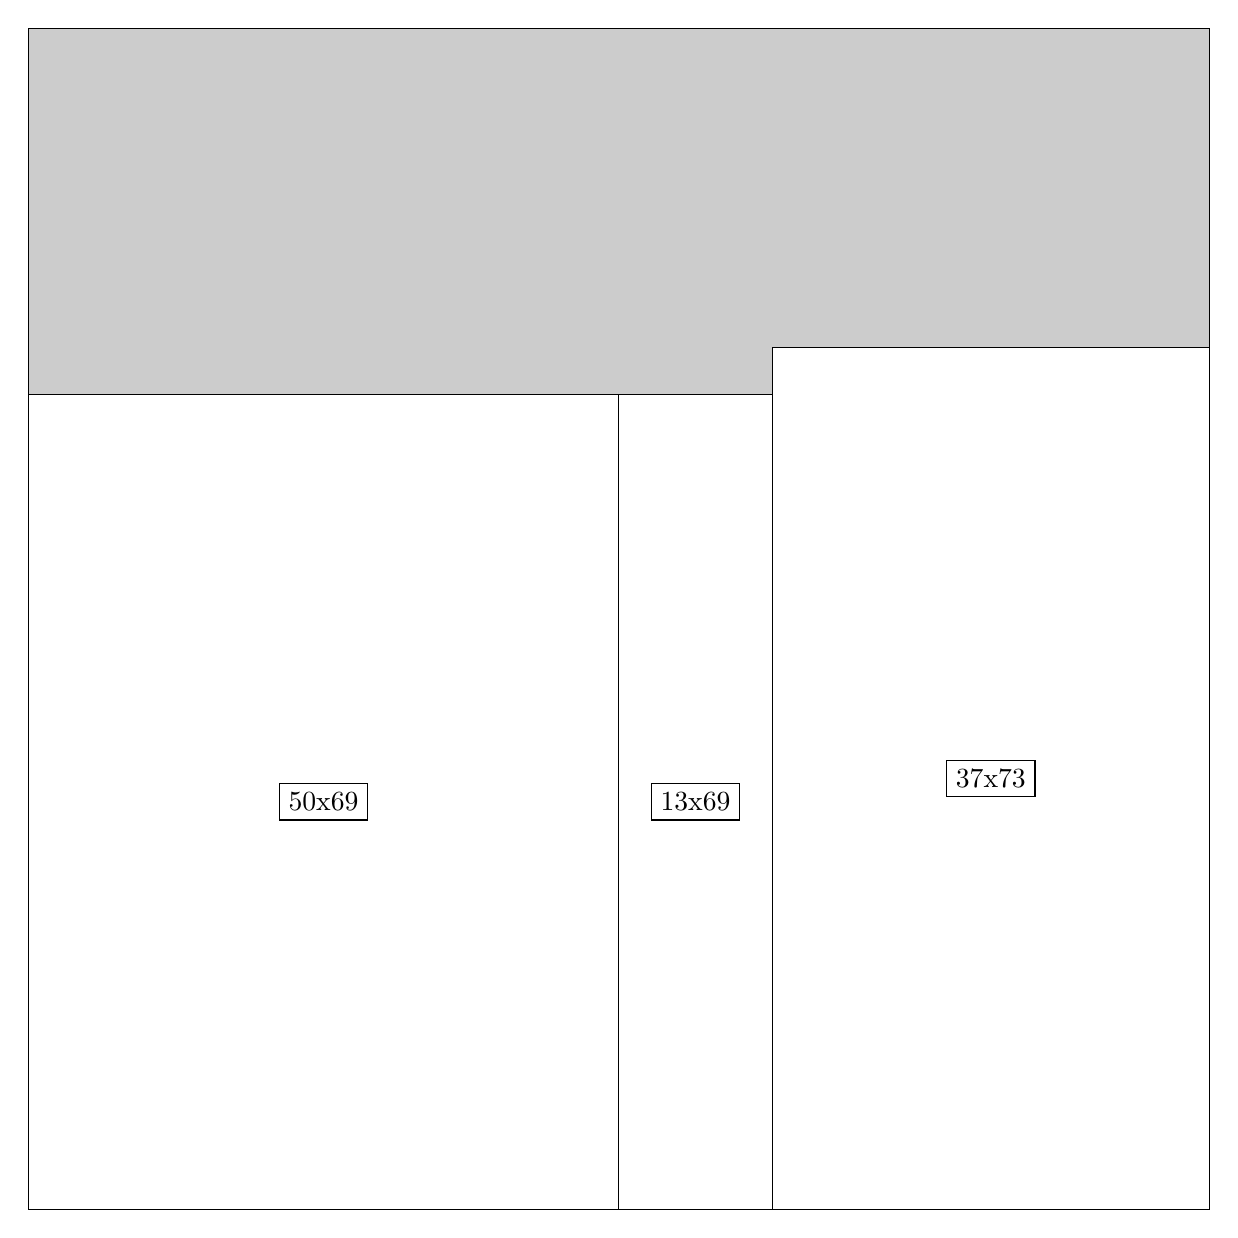
\begin{tikzpicture}[shorten >=1pt,scale=1.0,every node/.style={scale=1.0},->]
\tikzstyle{vertex}=[circle,fill=black!25,minimum size=14pt,inner sep=0pt]
\filldraw[fill=gray!40!white, draw=black] (0,0) rectangle (15.0,15.0);
\foreach \name/\x/\y/\w/\h in {50x69/0.0/0.0/7.5/10.35,37x73/9.45/0.0/5.55/10.95,13x69/7.5/0.0/1.95/10.35}
\filldraw[fill=white!40!white, draw=black] (\x,\y) rectangle node[draw] (\name) {\name} ++(\w,\h);
\end{tikzpicture}


w =50 , h =69 , x =0 , y =0 , v =3450
\par
w =37 , h =73 , x =63 , y =0 , v =2701
\par
w =13 , h =69 , x =50 , y =0 , v =897
\par
\newpage


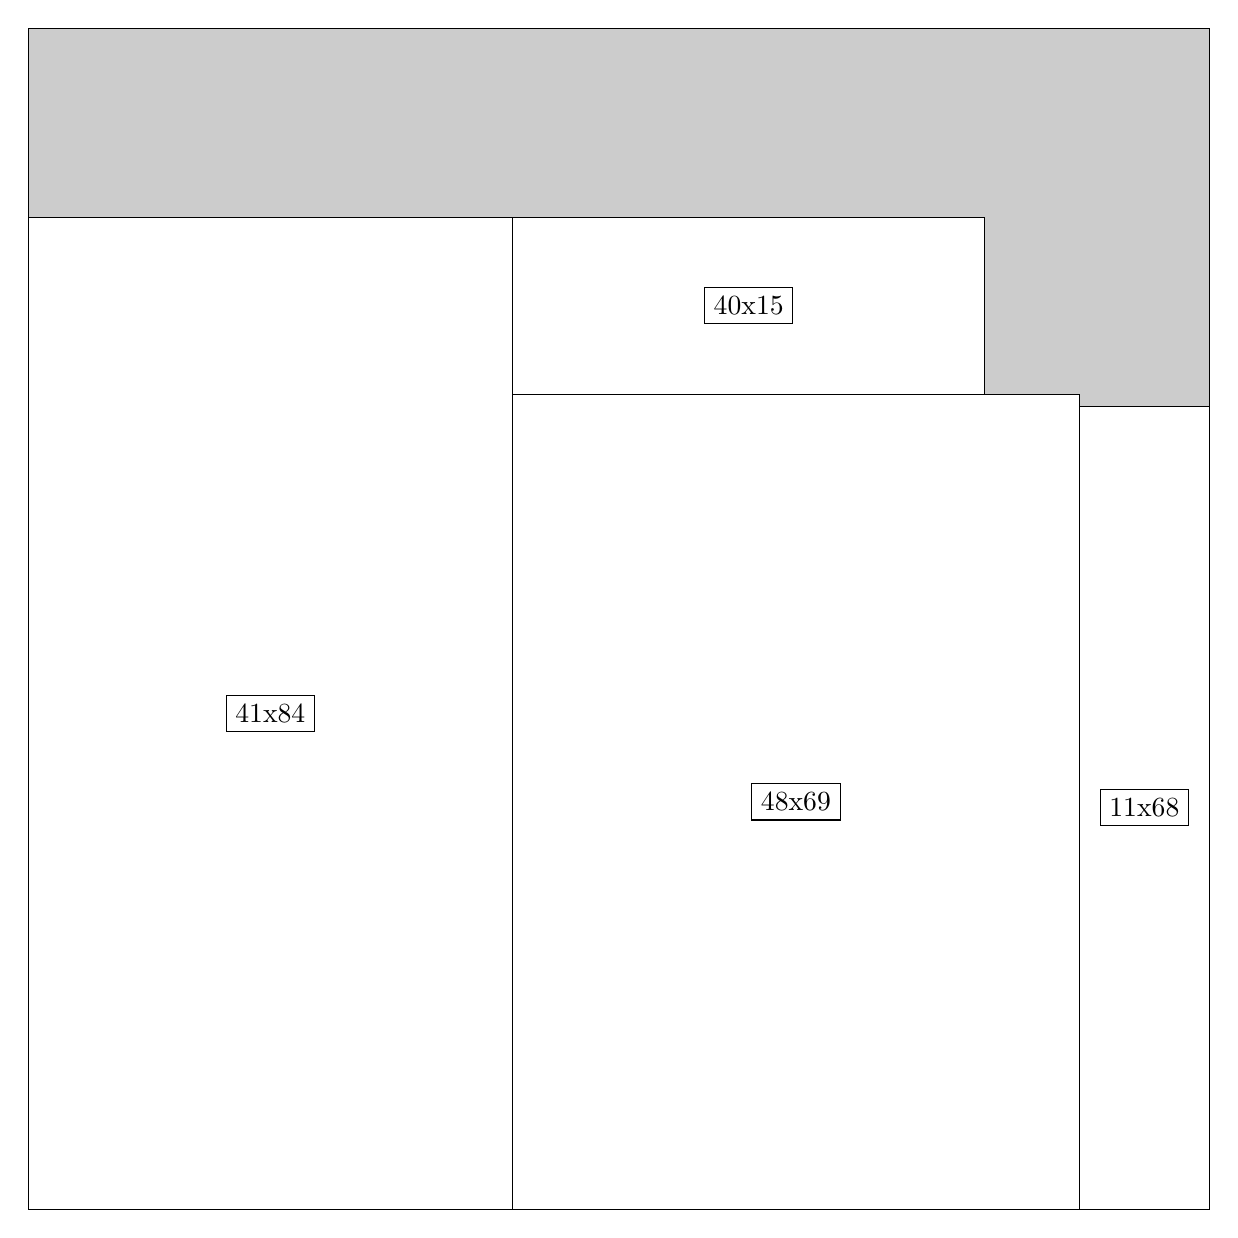
\begin{tikzpicture}[shorten >=1pt,scale=1.0,every node/.style={scale=1.0},->]
\tikzstyle{vertex}=[circle,fill=black!25,minimum size=14pt,inner sep=0pt]
\filldraw[fill=gray!40!white, draw=black] (0,0) rectangle (15.0,15.0);
\foreach \name/\x/\y/\w/\h in {41x84/0.0/0.0/6.1499999999999995/12.6,48x69/6.1499999999999995/0.0/7.199999999999999/10.35,11x68/13.35/0.0/1.65/10.2,40x15/6.1499999999999995/10.35/6.0/2.25}
\filldraw[fill=white!40!white, draw=black] (\x,\y) rectangle node[draw] (\name) {\name} ++(\w,\h);
\end{tikzpicture}


w =41 , h =84 , x =0 , y =0 , v =3444
\par
w =48 , h =69 , x =41 , y =0 , v =3312
\par
w =11 , h =68 , x =89 , y =0 , v =748
\par
w =40 , h =15 , x =41 , y =69 , v =600
\par
\newpage


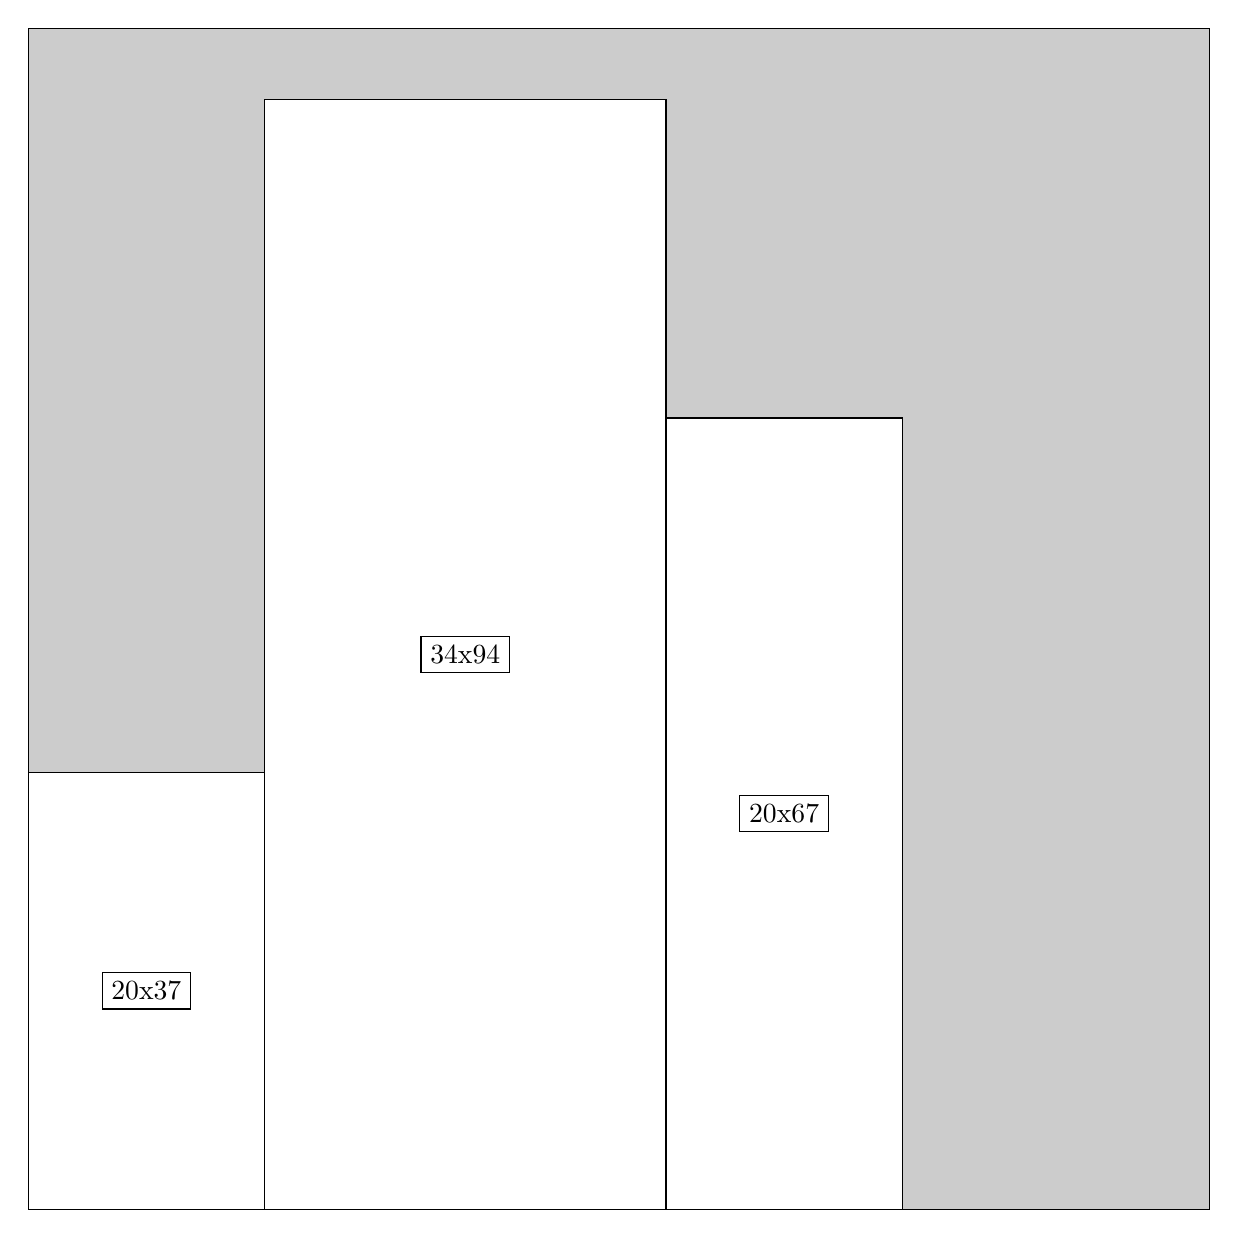
\begin{tikzpicture}[shorten >=1pt,scale=1.0,every node/.style={scale=1.0},->]
\tikzstyle{vertex}=[circle,fill=black!25,minimum size=14pt,inner sep=0pt]
\filldraw[fill=gray!40!white, draw=black] (0,0) rectangle (15.0,15.0);
\foreach \name/\x/\y/\w/\h in {34x94/3.0/0.0/5.1/14.1,20x67/8.1/0.0/3.0/10.049999999999999,20x37/0.0/0.0/3.0/5.55}
\filldraw[fill=white!40!white, draw=black] (\x,\y) rectangle node[draw] (\name) {\name} ++(\w,\h);
\end{tikzpicture}


w =34 , h =94 , x =20 , y =0 , v =3196
\par
w =20 , h =67 , x =54 , y =0 , v =1340
\par
w =20 , h =37 , x =0 , y =0 , v =740
\par
\newpage


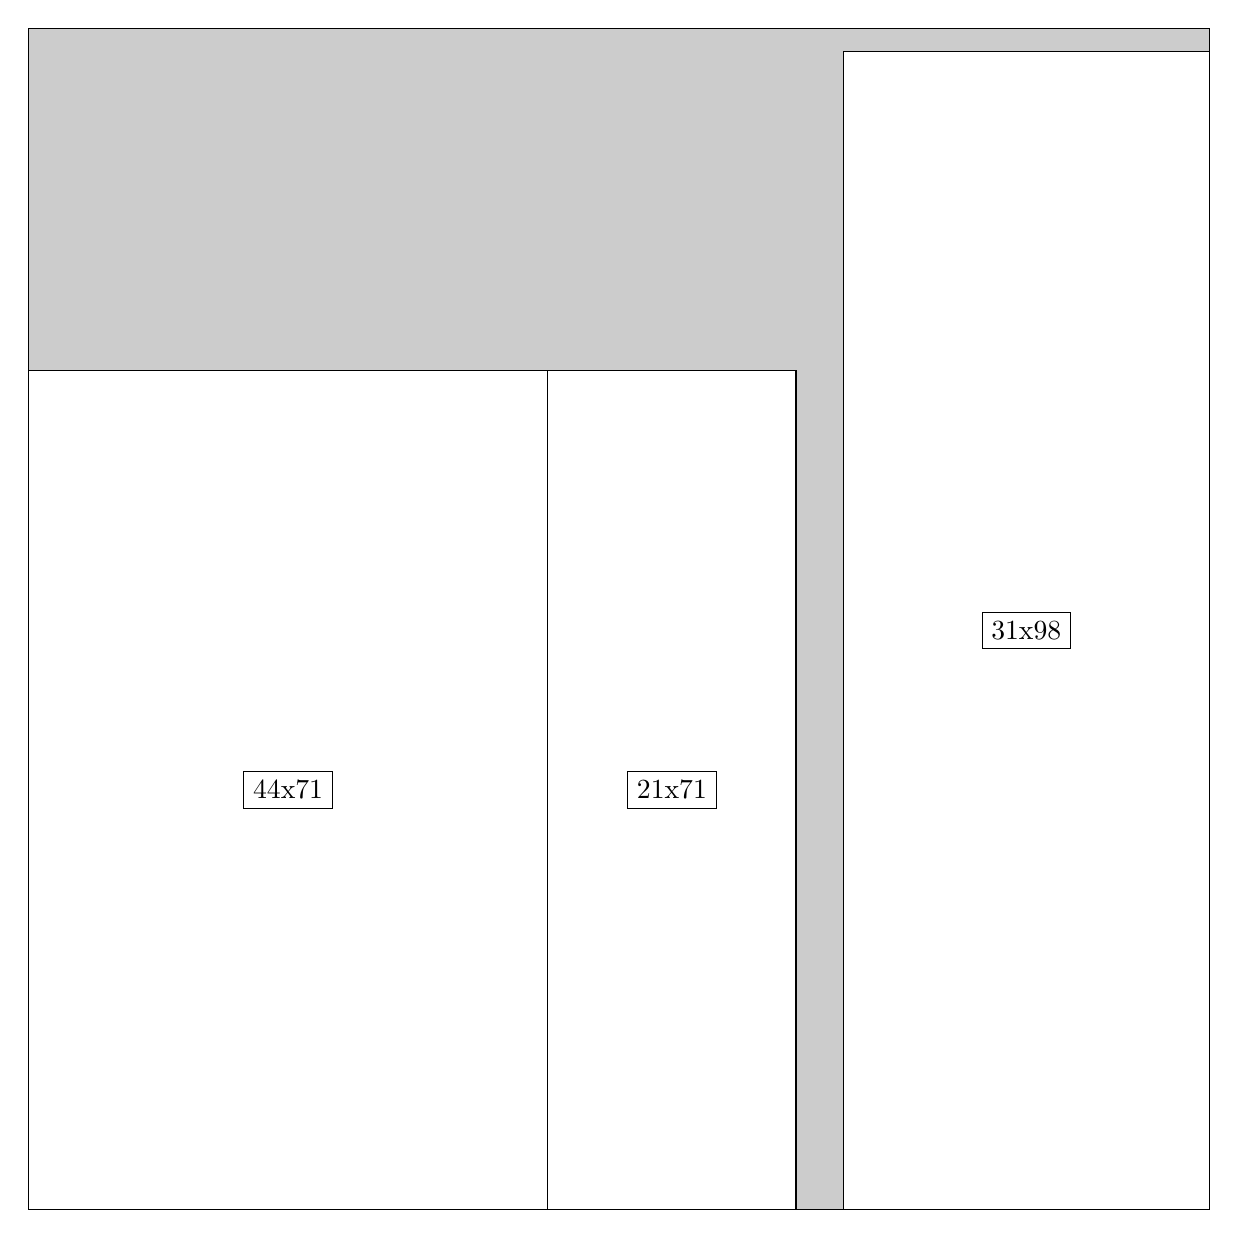
\begin{tikzpicture}[shorten >=1pt,scale=1.0,every node/.style={scale=1.0},->]
\tikzstyle{vertex}=[circle,fill=black!25,minimum size=14pt,inner sep=0pt]
\filldraw[fill=gray!40!white, draw=black] (0,0) rectangle (15.0,15.0);
\foreach \name/\x/\y/\w/\h in {44x71/0.0/0.0/6.6/10.65,31x98/10.35/0.0/4.6499999999999995/14.7,21x71/6.6/0.0/3.15/10.65}
\filldraw[fill=white!40!white, draw=black] (\x,\y) rectangle node[draw] (\name) {\name} ++(\w,\h);
\end{tikzpicture}


w =44 , h =71 , x =0 , y =0 , v =3124
\par
w =31 , h =98 , x =69 , y =0 , v =3038
\par
w =21 , h =71 , x =44 , y =0 , v =1491
\par
\newpage


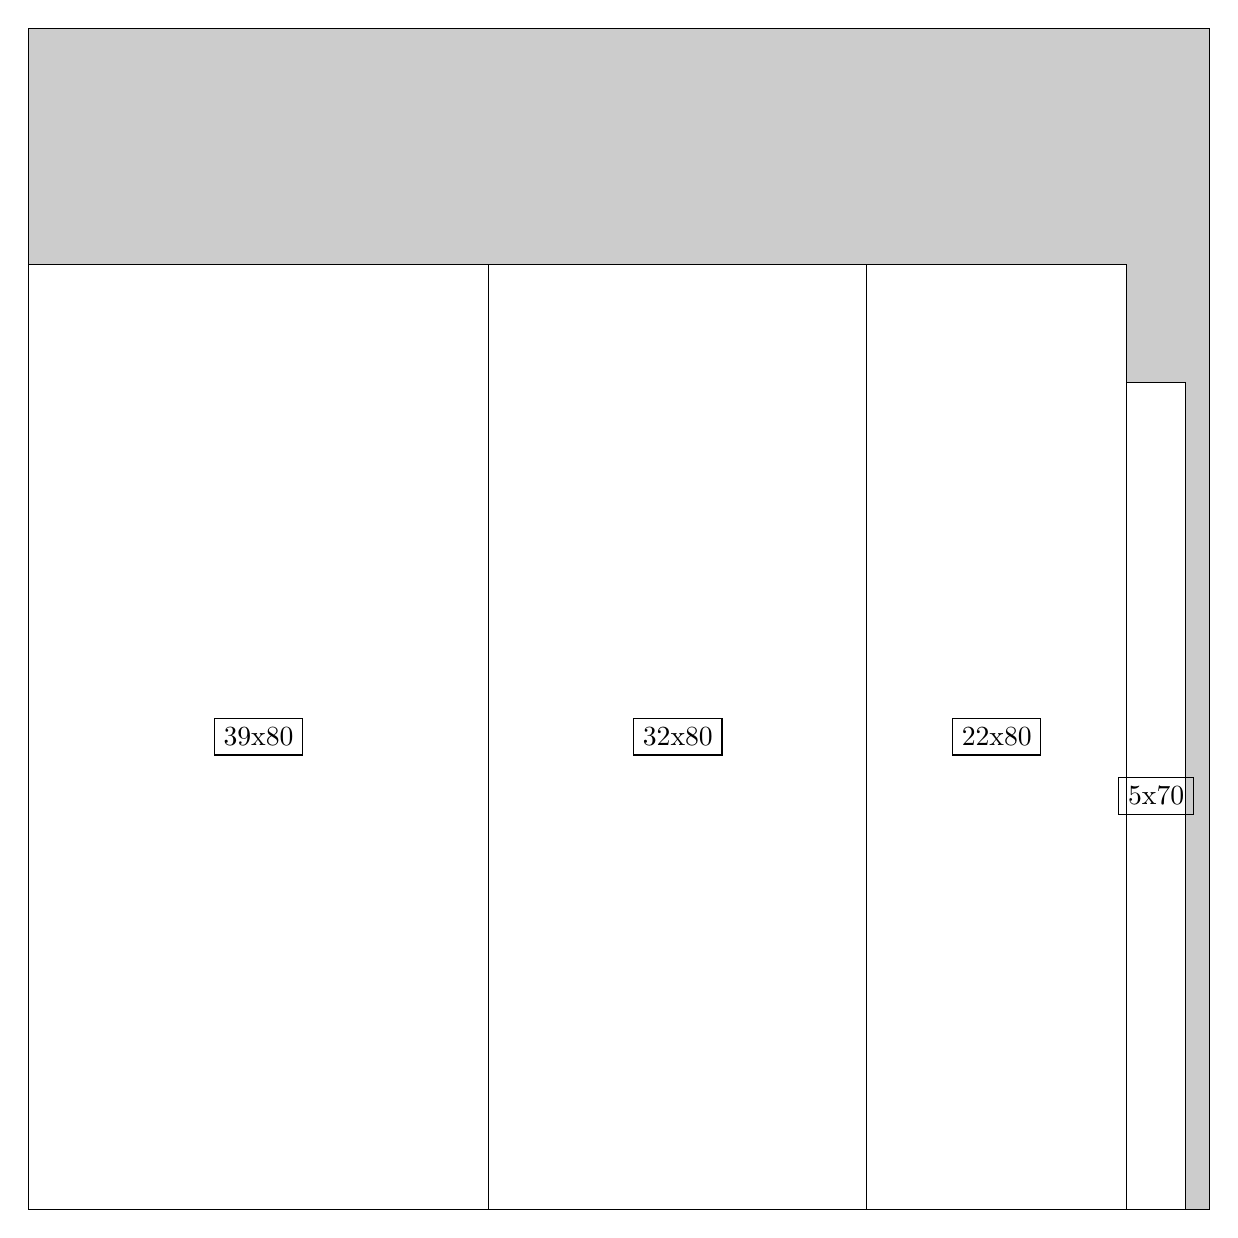
\begin{tikzpicture}[shorten >=1pt,scale=1.0,every node/.style={scale=1.0},->]
\tikzstyle{vertex}=[circle,fill=black!25,minimum size=14pt,inner sep=0pt]
\filldraw[fill=gray!40!white, draw=black] (0,0) rectangle (15.0,15.0);
\foreach \name/\x/\y/\w/\h in {39x80/0.0/0.0/5.85/12.0,32x80/5.85/0.0/4.8/12.0,22x80/10.65/0.0/3.3/12.0,5x70/13.95/0.0/0.75/10.5}
\filldraw[fill=white!40!white, draw=black] (\x,\y) rectangle node[draw] (\name) {\name} ++(\w,\h);
\end{tikzpicture}


w =39 , h =80 , x =0 , y =0 , v =3120
\par
w =32 , h =80 , x =39 , y =0 , v =2560
\par
w =22 , h =80 , x =71 , y =0 , v =1760
\par
w =5 , h =70 , x =93 , y =0 , v =350
\par
\newpage


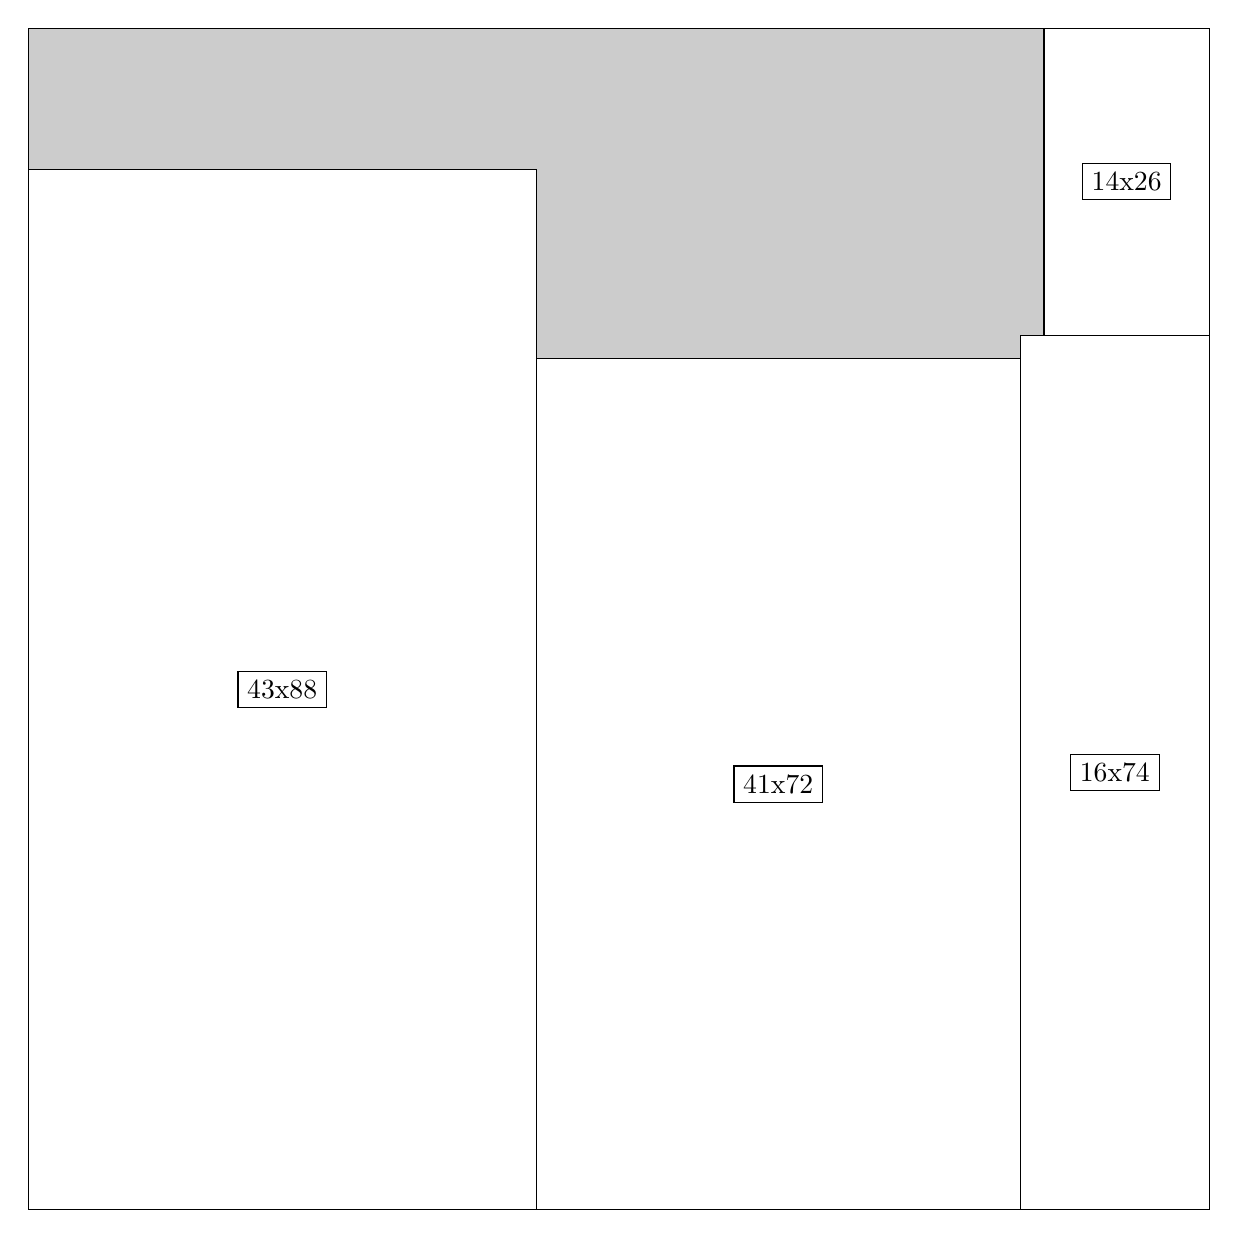
\begin{tikzpicture}[shorten >=1pt,scale=1.0,every node/.style={scale=1.0},->]
\tikzstyle{vertex}=[circle,fill=black!25,minimum size=14pt,inner sep=0pt]
\filldraw[fill=gray!40!white, draw=black] (0,0) rectangle (15.0,15.0);
\foreach \name/\x/\y/\w/\h in {43x88/0.0/0.0/6.45/13.2,41x72/6.45/0.0/6.1499999999999995/10.799999999999999,16x74/12.6/0.0/2.4/11.1,14x26/12.9/11.1/2.1/3.9}
\filldraw[fill=white!40!white, draw=black] (\x,\y) rectangle node[draw] (\name) {\name} ++(\w,\h);
\end{tikzpicture}


w =43 , h =88 , x =0 , y =0 , v =3784
\par
w =41 , h =72 , x =43 , y =0 , v =2952
\par
w =16 , h =74 , x =84 , y =0 , v =1184
\par
w =14 , h =26 , x =86 , y =74 , v =364
\par
\newpage


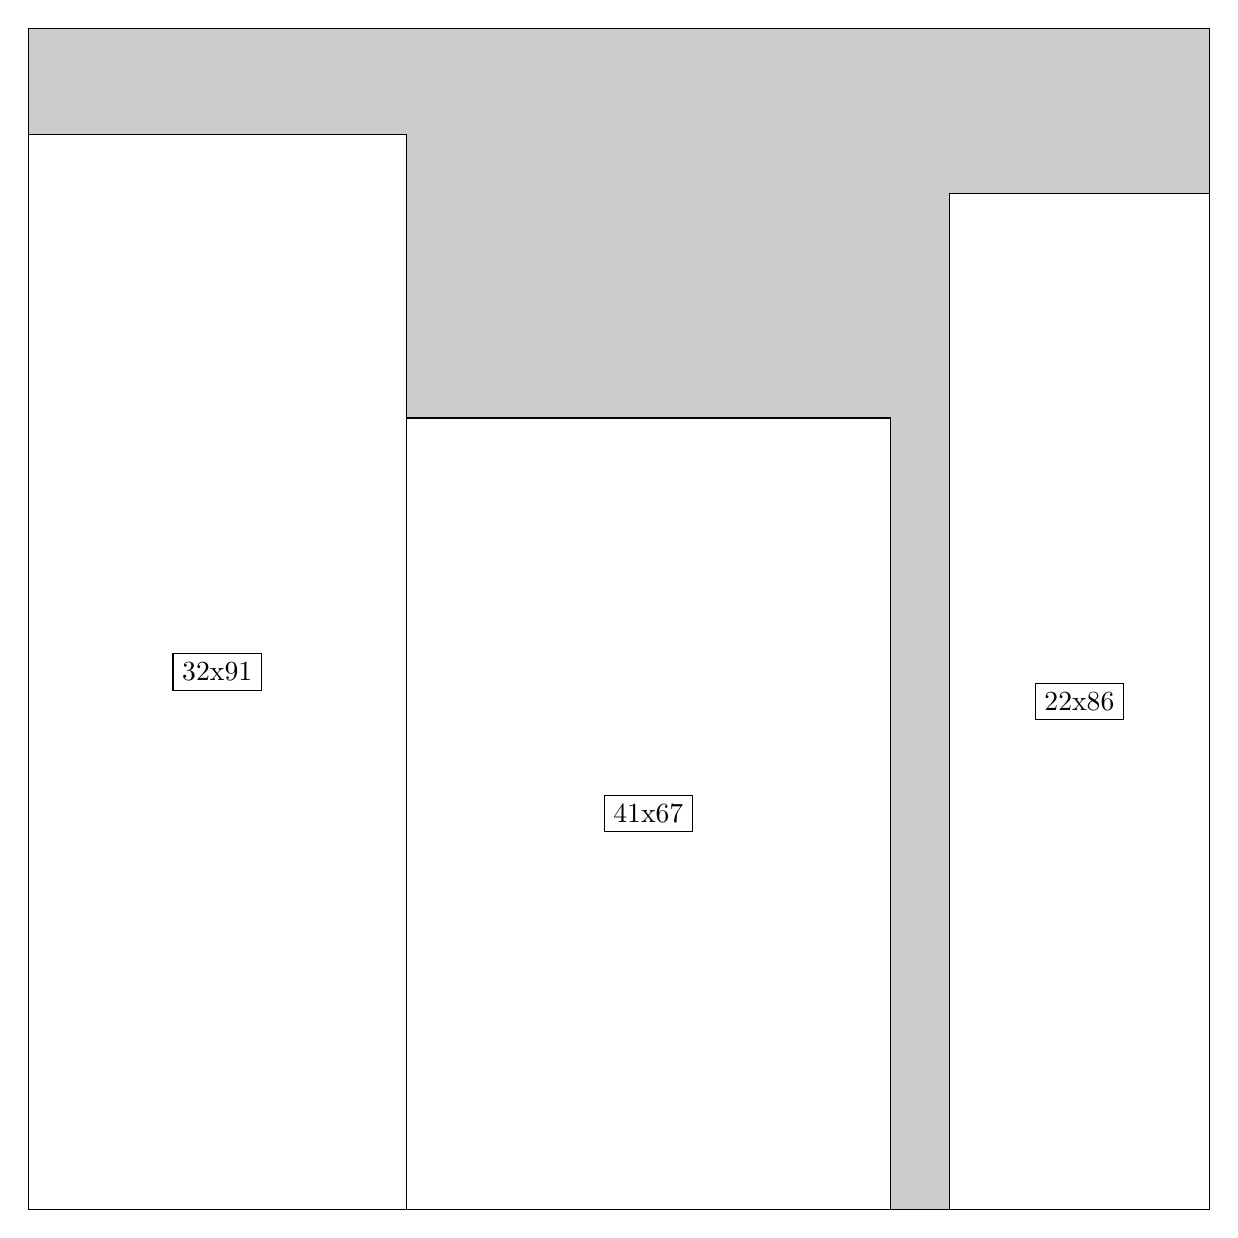
\begin{tikzpicture}[shorten >=1pt,scale=1.0,every node/.style={scale=1.0},->]
\tikzstyle{vertex}=[circle,fill=black!25,minimum size=14pt,inner sep=0pt]
\filldraw[fill=gray!40!white, draw=black] (0,0) rectangle (15.0,15.0);
\foreach \name/\x/\y/\w/\h in {32x91/0.0/0.0/4.8/13.65,41x67/4.8/0.0/6.1499999999999995/10.049999999999999,22x86/11.7/0.0/3.3/12.9}
\filldraw[fill=white!40!white, draw=black] (\x,\y) rectangle node[draw] (\name) {\name} ++(\w,\h);
\end{tikzpicture}


w =32 , h =91 , x =0 , y =0 , v =2912
\par
w =41 , h =67 , x =32 , y =0 , v =2747
\par
w =22 , h =86 , x =78 , y =0 , v =1892
\par
\newpage


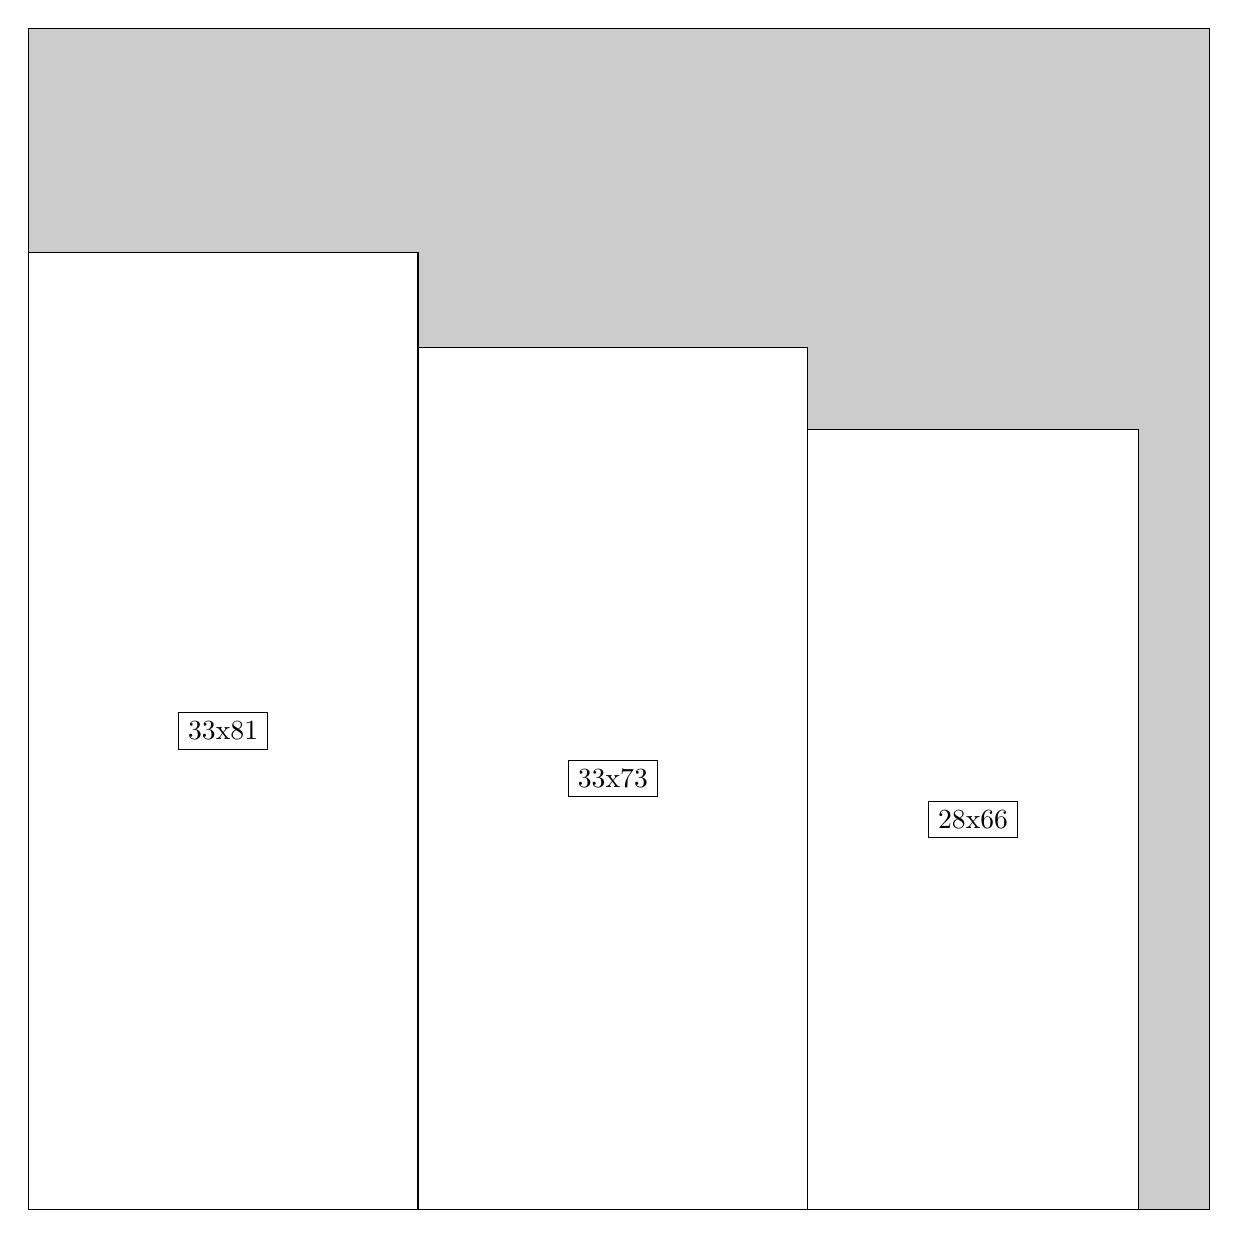
\begin{tikzpicture}[shorten >=1pt,scale=1.0,every node/.style={scale=1.0},->]
\tikzstyle{vertex}=[circle,fill=black!25,minimum size=14pt,inner sep=0pt]
\filldraw[fill=gray!40!white, draw=black] (0,0) rectangle (15.0,15.0);
\foreach \name/\x/\y/\w/\h in {33x81/0.0/0.0/4.95/12.15,33x73/4.95/0.0/4.95/10.95,28x66/9.9/0.0/4.2/9.9}
\filldraw[fill=white!40!white, draw=black] (\x,\y) rectangle node[draw] (\name) {\name} ++(\w,\h);
\end{tikzpicture}


w =33 , h =81 , x =0 , y =0 , v =2673
\par
w =33 , h =73 , x =33 , y =0 , v =2409
\par
w =28 , h =66 , x =66 , y =0 , v =1848
\par
\newpage


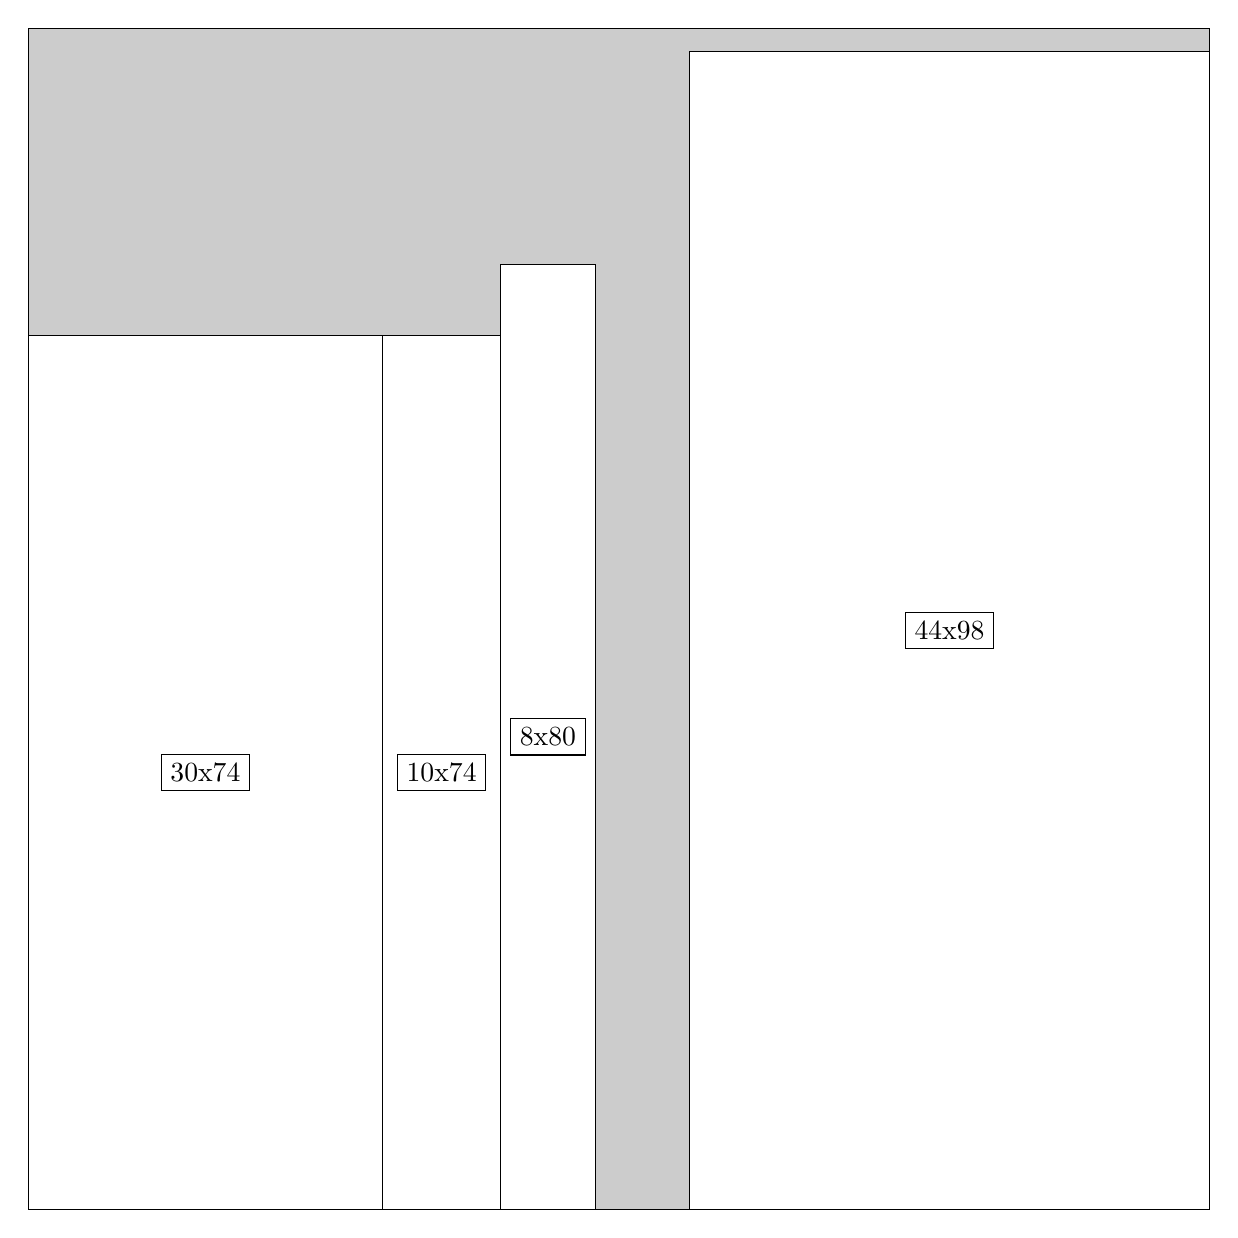
\begin{tikzpicture}[shorten >=1pt,scale=1.0,every node/.style={scale=1.0},->]
\tikzstyle{vertex}=[circle,fill=black!25,minimum size=14pt,inner sep=0pt]
\filldraw[fill=gray!40!white, draw=black] (0,0) rectangle (15.0,15.0);
\foreach \name/\x/\y/\w/\h in {44x98/8.4/0.0/6.6/14.7,8x80/6.0/0.0/1.2/12.0,30x74/0.0/0.0/4.5/11.1,10x74/4.5/0.0/1.5/11.1}
\filldraw[fill=white!40!white, draw=black] (\x,\y) rectangle node[draw] (\name) {\name} ++(\w,\h);
\end{tikzpicture}


w =44 , h =98 , x =56 , y =0 , v =4312
\par
w =8 , h =80 , x =40 , y =0 , v =640
\par
w =30 , h =74 , x =0 , y =0 , v =2220
\par
w =10 , h =74 , x =30 , y =0 , v =740
\par
\newpage


\end{document}